%%
%%  Hauptdatei
%%
%%  Projekt: Beispiel 
%%  Autor:   Arnemann
%%  Status:  
%%  Datum:   060814ar
%%           060815ar : Sperrvermerk und Zusammenfassung erg�nzt
%%           060830ar : v4 Anhang Seitennummerierung, viele Tabellen 
%%           060905ar : v5
%%           060908ar : v6
%%           060912ar : v6 FBMStyle_develop
%%           061025ar : v7 Richtlinentext entfernt
%%
%===================================================================
%% P R � A M B E L
%-------------------------------------------------------------------
%
%%==========================================================================================
%%
%% This is file 'FBMStyle_develop.tex'  v0.99
%%
%% Beta-Version eines Styles von M. Arnemann
%% basieren auf einem Muster von Herrn Kappler 
%% 060905ar
%% 060912ar
%%========================================================================================== 
\documentclass[
%        draft,                % Bilder nur mit Rahmen,  gut zur TextFehlersuche im dvi !!!!
        final,                % wenn es denn fertig ist.. 
        12pt,                 % Schriftgr��e (10pt, 11pt, 12pt) 11:pala, 10:Helv:ok, 
%        oneside,              % oneside f�r Draft 
        twoside,              % twoside
        onecolumn,            % Spalten (onecolumn/twocolumn)
%        twocolumn,
        pointlessnumbers,     % Kapitelnummer ohne . am Ende
        normalheadings,       % Groesse der Ueberschrift (bigheadings, normalheadings, smallheadings)
% Abs�tze
         halfparskip,         % Europ�ischer Satz mit Abstand zwischen Abs�tzen
%      
        idxtotoc,             % Index ins Verzeichnis einf�gen	*** pr�fen      
% Striche
%        headsepline,          % Strich unter Kopfzeile
        headinclude,          % Kopfzeile bei Satzspiegel bereucksichtigen
%        plainheadsepline,     % Strich auch beim Kapitelanfang (nicht ueblich)
%        footsepline,          % Strich ueber Fusszeile
%        footinclude,          % Fusszeile bei Satzspiegel beruecksichtigen
%        plainfootsepline,     % Strich auch beim Kapitelanfang
% Papier A4 (=Vorgabe) 
%        a4paper,              % Papier    
% Satzspiegel        
%        DIVcalc,              % Dichte des Druckes
%        DIVclassic,
%        DIV13,                % 8-15 f�r 11pt:std:10;  12pt:std:12, h�ngt vom Font ab !
                               % 13: mit palatino 11pt oder CM 12
         DIV15,                      
%        DIV15,                % mit palatino  12pt und Zeilenabstand > 1.2
        BCOR14mm ]            % Binderand  % 1mm, f�r Klebebindung % 14mm dann etwa gleichm��ig (Lochung)                                  % *** ! in der Datei f�r Titel ber�cksichtigen ! 
        {scrbook}             % Dokumenttyp // f�r Dipomarbeiten, Diss
%       {scrreprt}            % Dokumenttyp // Bericht bis etwa 80 Seiten
%       {scrartcl}            % Dokumenttyp // Seminararbeien 30 Seiten


%==============================================================================
%  PACKAGES
%==============================================================================
%\usepackage{calc}             % Rechnen innerhalb von Latex


%%-----------------------------------------------------------------------------
%% FONTS *** wird nichts aktiviert, dann gilt: Font Computer Modern ********
%       weitere Fonts: siehe online Help vom TechnicCenter: Font adttributes
%%-----------------------------------------------------------------------------

% - Ohne Serifen -           	% geht nicht
%\usepackage[scaled=.90]{helvet}	% etwas kleiner skaliert, damit es zu den anderen passt
%\usepackage{avant}          	% geht nicht
%\usepackage{garamond}
%
%% - Mit Serifen -
%\usepackage{times}          	% schmal
%\usepackage{mathptmx}       	% Times + passende Mathefonts

% *** den Vorschl�gen aus KOMA-Skript entsprechend, passt dieser Font
%     f�r die gew�hlte Textbreite am besten 
\usepackage{palatino}       	% breiter              **** sieht ganz gut aus 
%\usepackage{mathpazo}       	% passend zu palatino  **** 

%\usepackage{bookman}        	% breiter als palatino! 

%\usepackage{newcent}        	% for sophisticated font style
%\usepackage{lucid}          	% geht nicht
%
% -- Font Wahl (alternativ)
%
%\renewcommand{\familydefault}{phv}  % Adobe Helvetica 
%\renewcommand{\familydefault}{pag}  % AvantGarde-Book 
%\renewcommand{\familydefault}{ptm}  % Adobe Times (ziemlich eng)
%\renewcommand{\familydefault}{ppl}  % Palatino     (weiter) 
%\renewcommand{\familydefault}{pcr}  % Adobe Courier
%
% ** KOMA FONTS ** Schriften im Komaskript umdefinieren
%
%\setkomafont{chapter}{\rmfamily\huge}               % Chapter
%\setkomafont{section}{\rmfamily\Large}              % Section
%\setkomafont{subsection}{\rmfamily\large}           % subsection
%\setkomafont{subsection}{\rmfamily\normalsize}      % subsection
%
%\setkomafont{chapter}{\sffamily\huge}               % Chapter
%\setkomafont{section}{\sffamily\Large}              % Section
%\setkomafont{subsection}{\sffamily\large}           % subsection
%\setkomafont{subsection}{\sffamily\normalsize}      % subsection
%\setkomafont{pagehead}{\small\sffamily\slshape}     % Kopfzeile
%\setkomafont{pagenumber}{\bfseries\sffamily}        % Seitenzahl
%\setkomafont{sectioning}{\sffamily}                 % Titelzeilen
%\setkomafont{captionlabel}{\sffamily\bfseries\small}% Schrift f�r 'Abbildung' usw.
%\setkomafont{descriptionlabel}{\normalfont\bfseries}
%\addtokomafont{caption}{\sffamily\small\raggedright}% kleinere Schrift, linksb�ndig

\setkomafont{footnote}{\normalsize}                     % Marke und Text einer Fu�note
%\setkomafont{footnotelabel}{\normalsize}            %  
%\setkomafont{footnotereference}{\large}             % im Text
%
%%----------------------------------------------------------------------
%% Sprache
%%----------------------------------------------------------------------
%
\usepackage[T1]{fontenc}      % T1-encoded fonts: auch W�rter mit Umlauten trennen
\usepackage[T1]{url}          % much like \verb allow line breaks for paths and URLs
%\usepackage[OT1]{fontenc}    % Deutsche Umlaute im Text, klappt nicht immer gut
\usepackage[latin1]{inputenc} % Deutsche Umlaute: Eingabe nach ISO 8859-1 (Latin1)
                              % siehe Emacs: iso-accents-mode
%\usepackage[utf8]{inputenc}  % Eingabe nach UTF-8
%\usepackage{ae}              % almost european, virtueller T1-Font
\usepackage{ngerman}          % Neue deutsche Rechtschreibung

%%----------------------------------------------------------------------
%% Verschiedenes
%%----------------------------------------------------------------------
\usepackage[]{hyperref}         

\usepackage{latexsym}         		% Sonderzeichen
\usepackage{pifont}           		% dito
\usepackage{array}            		% f�r aufw�ndigere Tabellen
\usepackage{textcomp}        		% for upright mu (\textmu)
\usepackage[german=swiss]{csquotes}  % f�r quotes

%%----------------------------------------------------------------------
%% Satz (Seitenlayout)
%%----------------------------------------------------------------------
% -- Zeilenabstand vor typearea setzen! damit ganzzahlige Anzahl von Zeilen pro Seite
\usepackage{setspace}      	% Setzt Zeilenabstand  %\onehalfspacing
%\doublespace	         	% 2-facher Abstand
%\onehalfspace              	% 1,5-facher Abstand
\typearea                  	% nach der Schrift
        [current]          	% Heftrand BCOR oben definiert
%        {calc}             	% DIV neu berechnen aus package 
        {last}             	% DIV letzte aus Definition zuvor

\usepackage{multicol}      	% Mehrspaltiger Satz

%%----------------------------------------------------------------------
%% Kopf- und Fusszeilen
%%----------------------------------------------------------------------
\usepackage{scrpage2}          
%\pagestyle{scrheadings}            % Kopf- und Fusszeilen
%\clearscrheadfoot                  % Alles auf "" setzen

%% In [] steht, was am Kaptelanfang angezeigt wird, in {} steht,
%% was auf den uebrigen Seiten angezeigt wird. 
%% headmark = aktuelle Ueberschrift
%% pagemark = aktuelle Seite


%%%%% Kopf
%% ihead = Kopfzeile innen (links bei einseitigem Layout)
%%\ihead[]{innen}
%\ihead[\pagemark]{\pagemark}

%% chead = Kopfzeile mittig
%%\chead[]{mittig}

%% ohead = Kopfzeile aussen (rechts bei einseitigem Layout)
%\ohead[]{\headmark}


%%%%% Fuss
%% ifoot = Fusszeile innen (links bei einseitigem Layout)
%%\ifoot[]{innen}

%% cfoot = Kopfzeile mittig
%%\cfoot[]{mittig}

%% ofoot = Fusszeile aussen (rechts bei einseitigem Layout)
%%\ofoot[\pagemark]{\pagemark}
%


%%----------------------------------------------------------------------
%% Bilder , Grafiken
%%----------------------------------------------------------------------
%
\usepackage{epsfig,xspace}    	% PS Bilder
\usepackage{graphicx,color}   	% JPEG und PNG 
\usepackage{subfigure}	    		% Mehrere Bilder in einem mit ver. Bildunterschriften
%\usepackage{wrapfig}	     	% Text um Bild
%  \begin{wrapfigure}[12]{r}[34pt]{5cm} <figure> \end{wrapfigure}
%  [number of narrow lines] {placement} [overhang] {width of figure}
%  Placement is one of   r, l, i, o, R, L, I, O,  for right, left,
%  inside, outside, (here / FLOAT).
%
% *** nicht ben�tigt
%\usepackage[DVIPS]{graphicx,color}   % JPEG und PNG  f�r DVI
%\usepackage[pdftex]{graphicx,color} % pr�fen ob geht
%\usepackage{epstopdf}
%\usepackage[final]{graphicx}  % um Graphiken einzubinden (Wirkung kl�ren)


%%----------------------------------------------------------------------
%% Tabellen
%%----------------------------------------------------------------------
\usepackage{longtable}        	% seiten�bergreifende Tabellen passt zu KOMA
%\usepackage{supertab}         	% mehrseitige Tabellen
%% farbige Hyperlinks im PDF

%\usepackage{colortbl}        	% farbige Tabellen (v. D. Carlisle)
\usepackage{makeidx}          	% f�r Index-Erstellung 
\usepackage{listings}         	% f�r Latex Quelltext

%
%%----------------------------------------------------------------------
% Glossary
%%----------------------------------------------------------------------
%%% geht (noch) nicht  060830ar
%\usepackage[style=long,         % 
%            header=none,        %
%            border=none,        %
%            number=none,        %
%            cols=2,             %
%            toc=true]{glossary} % f�r Glossary 
%\usepackage{glossary} 
%\renewcommand{\glossaryname}{Glossar} %Damit nicht "`Glossary"' erscheint
%\makeglossary 

%%----------------------------------------------------------------------
%    Mathematik
%%----------------------------------------------------------------------
\usepackage[fleqn]{amsmath}
\usepackage{amssymb}
\usepackage{eqnarray}	    % nummerierte und unnummerierte Gleichungen/systeme

%%----------------------------------------------------------------------
%    Sonstiges
%%----------------------------------------------------------------------
%\usepackage{bm}              % for boldmath
%\usepackage{cite}
%\usepackage{url}
%   \urlstyle{rm}% for List of Contributors
%        
%\usepackage{format-thm}% some predefined theorem environments

%\usepackage{ragged2e}
%\usepackage{endnotes}
%\usepackage{xspace}

\usepackage{ifthen}
%\usepackage{eso-pic}  %add picture commands (or backgrounds) to every page
%\usepackage{afterpage}
%\usepackage{relsize}
%
%--- im Main-doc definieren
%\usepackage{chapterthumb}    % f�r Skripte: ChapterNummer am Rand
%\pagestyle{scrheadings}
%\lohead[\putchapterthumb]{\putchapterthumb}
%\addtokomafont{chapterthumb}{\bfseries}
%%
%%
%% other interesting packages:
%%
% \usepackage{varioref}
% \usepackage{verbatim}
% \usepackage{subfigure}
\usepackage{fancybox} % f�r schattierte ovale Boxen etc. geht nicht mit Miktex 5 060614ar
  %Command  	Effect \command{content to be boxed} 
  % fbox 	      square box
  % shadowbox 	square box with shadow
  % doublebox 	double square box
  % ovalbox 		thin oval box
  % Ovalbox 		thick oval box
%
% \usepackage{tabularx} % automatische Spaltenbreite
% \usepackage{supertab} % mehrseitige Tabellen

%----------------------------------------------------------------------
%% Satzspiegel = bedruckter Bereich
%%----------------------------------------------------------------------
% \usepackage{typearea}
%
%% Manuelle Einstellung des bedruckbaren Bereichs (NUR IM NOTFALL!)
% \areaset
%         [20mm]                % Heftrand
%         {150mm}               % Breite bedruckbarer Bereich
%         {237mm}               % H�he dito
%%
%% KOMA l�sst gerne oben zu wenig Rand
%% hiermit kann man den oberen Rand verschieben
% \setlength{\topmargin}{+3mm}  % gut mit Strich �ber Fusszeile


%% Einzug der ersten Zeile eines Absatzes. Im englischen Sprachraum
%% ist es �blich, einen neuen Absatz durch Einzug zu kennzeichnen.
%% Wir tun das �blicherweise durch einen gr��eren Zeilendurchschu�
%
%\setlength{\parskip}{3pt}               % Abstand von Absatz zu Absatz
%\setlength{\parindent}{0pt}             % Einzug 1. Zeile
%\setlength{\mathindent}{1em minus 1em} % f�r fleqn


%%
%%
%%  siehe Diplomarbeit von  Diplomarbeit mit LaTeX
%   Copyright (c) 2002-2005  Tobias Erbsland, Andreas Nitsch
%\usepackage[savemem]{listings} % f�r Listings
%\lstloadlanguages{TeX}


%----------------------------------------------------------------------
% Paket um Listings sauber zu formatieren.
% SUPER !
%----------------------------------------------------------------------
%\usepackage[savemem]{listings}
\usepackage{listings}
%\lstloadlanguages{LaTeX,Scilab,Delphi,Fortran,Matlab}

% ---------------------------------------------------------------------------
% Listing Definationen f�r PHP Code
% ---------------------------------------------------------------------------
\definecolor{lbcolor}{rgb}{0.85,0.85,0.85}
\lstset{language=[LaTeX]TeX,
	numbers=left,
	stepnumber=1,
	numbersep=5pt,
	numberstyle=\tiny,
	breaklines=true,
	breakautoindent=true,
	postbreak=\space,
	tabsize=2,
	basicstyle=\ttfamily\footnotesize,
	showspaces=false,
	showstringspaces=false,
	extendedchars=true,
	backgroundcolor=\color{lbcolor}}

% ---------------------------------------------------------------------------
% footnote
% ---------------------------------------------------------------------------
%\deffootnote[1em]{1.5em}{1em}{\textsuperscript{\thefootnotemark}} % std
\deffootnote{1em}{1.5em}{\textsuperscript\thefootnotemark\ } %Text klebt nicht an Zahl

% ---------------------------------------------------------------------------
% Neue Umgebungen
% ---------------------------------------------------------------------------
\newenvironment{ListChanges}%
	{\begin{list}{$\diamondsuit$}{}}%
	{\end{list}}
%
%% **** END OF CLASS MStyle ****


%%%==========================================================================================
%%
%% This is file 'FBMStyle.tex'  v0.98
%% see also file 'FBMStyle_develop.tex
%%
%% Beta-Version eines Styles von Michael Arnemann
%% basieren auf einem Muster von Uwe Kappler 
%% 060905ar
%%========================================================================================== 
\documentclass[
        final,                % wenn es denn fertig ist.. 
        12pt,                 % Schriftgr��e (10pt, 11pt, 12pt) 11:pala:ok, 
        twoside,              % oneside, twoside
        pointlessnumbers,     % Kapitelnummer ohne . am Ende
        normalheadings,       % Groesse der Ueberschrift (bigheadings, normalheadings, 
        halfparskip,          % Europ�ischer Satz mit Abstand zwischen Abs�tzen
        idxtotoc,             % Index ins Verzeichnis einf�gen	*** pr�fen      
        headsepline,          % Strich unter Kopfzeile
        headinclude,          % Kopfzeile bei Satzspiegel bereucksichtigen
        DIV13,                % mit palatino 11pt oder CM 12
        BCOR14mm]             % Binderand    %1mm, f�r Klebebindung % 14mm dann etwa gleichm��ig
   {scrbook}                  % Dokumenttyp // f�r Dipomarbeiten, Diss
%----------------------------------------------------------------------------------------
%  PACKAGES
%----------------------------------------------------------------------------------------
\typearea                  % nach der Schrift
        [current]          % Heftrand BCOR oben definiert
%        {calc}             % DIV neu berechnen aus package 
        {last}             % DIV letzte aus Definition zuvor

%\usepackage{scrpage2}        % Package laden 
\usepackage[light,math]{iwona}
\usepackage[T1]{fontenc}     % T1-encoded fonts: auch W�rter mit Umlauten trennen
\usepackage[T1]{url}         % much like \verb allow line breaks for paths and URLs
\usepackage[latin1]{inputenc} % Deutsche Umlaute: Eingabe nach ISO 8859-1 (Latin1)
\usepackage{epsfig,xspace}    % PS Bilder
\usepackage{graphicx,color}   % JPEG und PNG 
\usepackage{subfigure}	    % Mehrere Bilder in einem mit ver. Bildunterschriften
\usepackage{wrapfig}	    % Text um Bild

\usepackage[]{hyperref}         
\usepackage{ngerman}          % Neue deutsche Rechtschreibung
\usepackage{latexsym}         % Sonderzeichen
\usepackage{pifont}           % dito
\usepackage{array}            % f�r aufw�ndigere Tabellen
\usepackage{longtable}        % seiten�bergreifende Tabellen passt zu KOMA
\usepackage{multicol}         % Mehrspaltiger Satz
\usepackage{makeidx}          % f�r Index-Erstellung 
\usepackage{listings}         % f�r Latex Quelltext
\usepackage{textcomp}        % for upright mu (\textmu)
\usepackage[german=swiss]{csquotes}  % f�r quotes
\usepackage[fleqn]{amsmath}
\usepackage{amssymb}
\usepackage{eqnarray}	    % nummerierte und unnummerierte Gleichungen/systeme
\usepackage{ifthen}
\usepackage{fancybox} % f�r schattierte ovale Boxen etc. geht nicht mit Miktex 5 060614ar
%----------------------------------------------------------------------
% Paket um Listings sauber zu formatieren.
% SUPER !
%----------------------------------------------------------------------
\usepackage{listings}
% ---------------------------------------------------------------------------
% Listing Definationen f�r PHP Code
% ---------------------------------------------------------------------------
\definecolor{lbcolor}{rgb}{0.85,0.85,0.85}
\lstset{language=[LaTeX]TeX,
	numbers=left,
	stepnumber=1,
	numbersep=5pt,
	numberstyle=\tiny,
	breaklines=true,
	breakautoindent=true,
	postbreak=\space,
	tabsize=2,
	basicstyle=\ttfamily\footnotesize,
	showspaces=false,
	showstringspaces=false,
	extendedchars=true,
	backgroundcolor=\color{lbcolor}}

% ---------------------------------------------------------------------------
% Neue Umgebungen
% ---------------------------------------------------------------------------
\newenvironment{ListChanges}%
	{\begin{list}{$\diamondsuit$}{}}%
	{\end{list}}
%
%% **** END OF CLASS MStyle ****
%
%****
%%----------------------------------------------------------------------
%% pdf-setup 060830ar
%%----------------------------------------------------------------------
%
%

\hypersetup{%
  %backref,%
  pdftitle    = {Richtlinien zur Durchf�hrung von Abschlussarbeiten},
  pdfsubject  = {Fakult�t f�r Wirtschaftsinformatik},
  pdfauthor   = {Prof. Dr.-Ing. M. Arnemann},
  pdfkeywords = {Richtlinie, Abschlu�arbeit, Bericht},
%  pdfcreator  = {Adobe-Acrobat-Distiller},
%  pdfproducer = {LaTeX with hyperref und thumbpdf},
  pdfpagemode  = UseThumbs, % Anzeige Piktogramme
  bookmarksopen = true,     % Anzeige aller Ebenen
  bookmarksnumbered = true, % Anzeige Abschnittsnummern  
  pdfstartpage = {1}        % Startseite, hilfreich mit pdf
 }
% 

\hypersetup{%
%  pagebackref,
  bookmarksnumbered,
%  backref,
%  bookmarks,
%  breaklinks,
%  linktocpage,
%
%alternative Farbwahl
%  colorlinks  = true,
%  linkcolor   = blue,
%  urlcolor    = red,
%  tocdepth     = 3            
}
             
%%
%% wenn f�r alles die gleiche Farbe ..
%%
%\definecolor{LinkColor}{rgb}{0,0,0.5} %duckelblau
%\definecolor{LinkColor}{rgb}{0,0,1} %blau
%\definecolor{LinkColor}{rgb}{0.5,0,0} % dunkelrot bis braun
%\definecolor{LinkColor}{rgb}{1,0,0} % rot
\definecolor{LinkColor}{rgb}{0.7,0,0} % kr�ftig rot
\hypersetup{%
  colorlinks=true,%
	linkcolor=LinkColor,%
	citecolor=LinkColor,%
	filecolor=LinkColor,%
	menucolor=LinkColor,%
	pagecolor=LinkColor,%
	urlcolor=LinkColor
}

%
% Makros       
% 060911ar
% 060926ar evtl. Unterschied zu Richtlinie
%******************************************************************************


%%=============================================================================
%% Neue, neudefinierte Befehle
%%=============================================================================

%-------------------------------------------------------------------
% Abbildungen **** Empfehlung: Kopiervorlage nutzen und anpassen, nicht Makro!
%-------------------------------------------------------------------
% Vorsicht: Dateinamen in UNIX-Syntax und relativ zu main.tex
%
% Syntax gilt f�r alle unterst�tzten Grafikformate!
% Voraussetzung: die Datei existiert und die Endung wird NICHT 
% im Dateinamen angegeben!
%
% Syntax: 
% \fg {DATEINAME}% = caption
%          {Ort auf Blatt} htbf
%          {BREITE} % vorzugsweise als Teil der TExtbreite z.B. '0.8\textwidth'
%          {ROTATIONSWINKEL}%
%          {Bildtitel im Abbildungsverzeichnis}
%          {BILDUNTERSCHRIFT}%
%
% Kopiervorlage 
% \fg{Datei}{Ort}{Breite}{Rotation}{Bildtitel im Abbildungsverzeichnis}{Bildunterschrift}%

\newcommand{\fg}[6]
             {
              \begin{figure}[#1]
              \begin{center}
              \includegraphics[width=#3, angle=#4]{#2}
              \caption[#4]{%
              \label{fig:#2}%
              #5}
              \end{center}
              \end{figure}
             }

             
%-------------------------------------------------------------------
% Abbildungen caption beside
%-------------------------------------------------------------------
% Kopiervorlage: in den Quelltext kopieren, dann dort umbrechen
%\fgB{Datei}{Ort, !h oder tbh}{Breite}{Rotation}{Bildunterschrift}{i}{Text}
%
% Syntax: 
%\fgB {DATEINAME}
%        {Ort, !h oder tbh}   
%        {BREITE} % vorzugsweise als Teil der TExtbreite z.B. '0.8\textwidth'
%        {ROTATIONSWINKEL}
%        {BILDUNTERSCHRIFT}
%        {Ausrichtung Caption= i oder o}
%        {Text im Abbildungsverzeichnis}
%
% Vorsicht: Dateinamen in UNIX-Syntax und relativ zu main.tex
% evtl ist der Abstand zwischen Text und Bild zu klein
% dann �ndern (siehe Koma skript  
\newcommand{\fgB}[7]
             {
              \begin{figure}[#2]
              %\setcapindent*{1em}  %h�ngender Einzug ab 2. Zeile
              \begin{captionbeside}[#7]%
              {#5}[#6][\linewidth]%
              %[2em]* %Verschiebung nach aussen
              \includegraphics[width=#3, angle=#4]{#1}
              \end{captionbeside}%              
              \label{fig:#1}
              \end{figure}
             }             
%-------------------------------------------------------------------
% Tabellen
%-------------------------------------------------------------------
% Syntax: \bt{SPALTENDEFINITION} - Begin Table
%         \et{LABEL}{TABELLENBEZEICHNUNG}
\newcommand{\bt}[3]
           { 
             \begin{table}[!h]
             \begin{center}
             \caption{\label{tbl:#2}#3}                          
             \begin{tabular}{#1}
           }
\newcommand{\et}
           {
            \end{tabular}
            \end{center}
            \end{table}
           }


%%=============================================================================
%% Abk�rzungen (Abteilung "Faulheit")
%%=============================================================================
%
% --- Gleichungen 
% Syntax: \beq{NAME DER GLEICHUNG} 
%         \eeq
% Referenz: \ref{eqt:NAME DER GLEICHUNG}
%
% begin
\newcommand{\beq}[1]
           {
            \begin{equation}
            \label{eqt:#1}
           }
% end
\newcommand{\eeq}
           {
             \end{equation}
           }
\newcommand{\beqa}{\begin{eqnarray}}         
\newcommand{\eeqa}{\end{eqnarray}}

\newcommand{\ba}{\begin{array}}
\newcommand{\ea}{\end{array}}

\newcommand{\bdm}{\begin{displaymath}}
\newcommand{\edm}{\end{displaymath}}
	   
% --- Itemize 
\newcommand{\bi}{\begin{itemize}}
\newcommand{\ei}{\end{itemize}}

% --- Enumerate
\newcommand{\be}{\begin{enumerate}}
\newcommand{\ee}{\end{enumerate}}

% ---
\newcommand{\bd}{\begin{description}}
\newcommand{\ed}{\end{description}}

% Fussnoten
% Syntax: \fn legt fest, wo das Fu�notenzeichen steht
%         \fnt{FUSSNOTENTEXT} legt den Text fest
\newcommand{\fn}{\footnotemark}
\newcommand{\fnt}[1]{\footnotetext{#1}}

\newcommand{\s}{\scriptscriptstyle}
\newcommand{\D}{\displaystyle}

\newcommand{\ol}{\ddot{O}l}
\newcommand{\p}{\partial}
\newcommand{\Dp}{\Delta p}
\newcommand{\te}{$\vartheta$}             % theta
\newcommand{\R}{{\em\bf R}}               % Universelle Gaskonstante fett
\newcommand{\C}{$^\circ$C}                % Grad Celsius
\newcommand{\mue}{\textmu}
\renewcommand{\d}{\partial\mspace{2mu}}   % partielles Diff. Zeichen 
\newcommand{\td}{\,\mathrm{d}}           	% totales Diff (d, nicht kursiv)
\newcommand{\ddt}[1]{\frac{\td #1}{\td t}}% zweifach 

\newcommand{\idx}[1]{_\mathrm{#1}}        % nicht kursiver Index in Gleichungen geht nur mit Umlauten wie "a


\newcommand{\bul}{$\bullet$}              % Mark in Tabs
\newcommand{\Q}{$\bullet$}                % mark2 in Tabs
\newcommand{\mc}{\multicolumn}


\def\zB{z.\,B.\ }
\def\dh{d.\,h.\ }
\def\ua{u.\,a.\ }
\def\su{s.\,u.\ }
\newcommand{\bzw}{bzw.\ }
%%
%% Refrenzen
%%
%\newcommand{\RefTab}[1]{$\underline{\mbox{Tab.~\ref{#1}}}$}   % 1. Tabellenref. im Text
%\newcommand{\RefFig}[1]{$\underline{\mbox{Abb.~\ref{#1}}}$}   % 1. Bildref.
\newcommand{\RefTab}[1]{\textbf{Tabelle~\ref{#1}}}             % 1. Tabellenref. im Text
\newcommand{\RefFig}[1]{\textbf{Bild~\ref{#1}}}                % 1. Bildref.
\newcommand{\RefTabc}[1]{Tabelle~\ref{#1}}                        % 2. Tabellenref. im Text
\newcommand{\RefFigc}[1]{Bild~\ref{#1}}                        % 2. Bildref.

\newcommand{\RefEq}[1]{\mbox{Gl.~(\ref{#1})}}                  % Gleichungen

\newcommand{\ZmE}[2]{$#1$~{#2}}                                % Zahl:#1 mit Einheiten#2 #3
\newcommand{\EH}[1]{#1}                                        %  Einheiten
\newcommand{\B}[1]{\mbox{#1}}

%-------------------------------------------------------------

\newfont{\ssf}{cmss10 scaled 1000}
\newfont{\ssb}{cmssbx10 scaled 1000}

\newcommand{\cf}{\ssf}                 % CaptionFonts: in Bildunter- ,Tab�berschriften
\newcommand{\rf}{\em}                  % RefFonts    : Kennzeichnung von Referenzen im Text
\newcommand{\eng}{\tt}                 % englische Begriffe im deutschne Text 

% Hinweis
% Syntax: \oops{�BERSCHRIFT}{TEXT}
%        : nach �berschtift wird automatisch eingef�gt
\newcommand{\oops}[2]{\begin{quote}\textbf{#1}:\\ {#2} \end{quote} }


%---------------------------------------------------------------
% Bildunter- und Tabellen�berschriften
%---------------------------------------------------------------
% z.B. andere Schrift, oder auch Schriftform und andere Abk�rzung
%
% alternaiv : "Abbildungen" lassen und
%  Zeilenumbruch bei Bildbeschreibungen einf�hren \setcapindent{1em}
%
% bessere Methoden: siehe Komaskript
\def\figurename{Bild}          % oder: Bild z.B. {\bfseries Abb.}
%\def\tablename{Tab.}          % oder: z.B. Tafel, Tab.

\renewcommand*{\captionformat}{.~} % DIN l�sst gr�ssen
%\addtokomafont{caption}{\sffamily\small\raggedright}  % kleinere Schrift, linksb�ndig
\addtokomafont{caption}{\sffamily\small}  % kleinere Schrift
%\setkomafont{descriptionlabel}{\sffamily\small}
\setkomafont{captionlabel}{\sffamily\bfseries}
\setcaphanging
\setcapindent{0em}             % kein Einzug


%---------------------------------------------------------------
% Literaturliste: Formatierung der Liste wird HIER vorgenommen!
%---------------------------------------------------------------
\newcommand{\lit}[4]
           {
              \bibitem{#1}
                 {#2:}
                 #3 
                 #4 
           }

%---------------------------------------------------------------
%
%---------------------------------------------------------------
% Kommentare 
\newcommand{\Kommentar}[1]{{\em #1}} 


% Verstecktes
% Alles innerhalb von \Hide{} oder \ignore{}
% wird von LaTeX komplett ignoriert (wie ein Kommentar)
\newcommand{\Hide}[1]{}
\let\ignore\Hide



         % Macros lagen
%%-----------------------------------------------------------------
% Beschriftung des Titelblatts - Vorderseite
%-------------------------------------------------------------------
\pagestyle{scrheadings}            % Kopf- und Fusszeilen
\clearscrheadfoot                  % Alles auf "" setzen
\setcounter{page}{1}       		  % anpassen: wenn 1 Seitig  dannn 2     
\pagenumbering{roman}

\usepackage{001_Titel/0011_TitlePage-HsKa_Setup/HsKAtitle12}
\department{Fakult�t f�r Wirtschaftsinformatik}

\title{Mustertitel erste  Zeile\\ % Titel erste  Zeile
       Titel zweite Zeile\\ % Titel zweite Zeile
       \vspace*{1em}		 % Titel dritte Zeile
       4.  Zeile% Titel vierte Zeile
      } 
\thesistype{*Diplomarbeit}  % Masterthesis o.�
\thesisno{*D 06/01}

\author{*Vorname Nachname}
\BDate{*Geburtstag}
\BLocation{*Geburtsort}
\matno{*1234567}


\companyname{*Organisation}
\tutor{*1. Organisation}{*2. Hochschule}
\location{*Karlsruhe}
\duration{*01. 08. 2006   bis  31. 01. 2007}

\restrictionnotice{*S P E R R V E R M E R K}      
\restrictionnotice{*** V E R T R A U L I C H ***}      
%%
% Bemerkung auf der R�ckseite, wenn zweiseitig
%
\Schriftsatz{%
    Satz und Herstellung:\\
    {\LaTeX} und KomaSkript  /  MiKTeX 2.5, TeXnicCenter 1 Beta 7.01.\\
    Font: Computer Modern, 12 pt\\
    Druckdatum: \today
    }%     
%-----------------------------------------------------------------
% Beschriftung des Titelblatts - Vorderseite
%-------------------------------------------------------------------
\pagestyle{scrheadings}            % Kopf- und Fusszeilen
\clearscrheadfoot                  % Alles auf "" setzen
\setcounter{page}{1}       		  % anpassen: wenn 1 Seitig  dannn 2     
\pagenumbering{roman}

\usepackage{001_Titel/0011_TitlePage-HsKa_Setup/HsKAtitle12}
\department{Fakult�t f�r Wirtschaftsinformatik}
%\course{Studiengang Wirtschaftinformatik}

\thesistype{Bachelorthesis}  % Masterthesis o.�
\author{*Vorname Nachname}

\title{Mustertitel erste  Zeile} 

\thesisno{*D 06/01}


\BDate{*Geburtstag}
\BLocation{*Geburtsort}
\matno{*1234567}


\companyname{*Organisation}
\tutor{*1. Organisation}{*2. Hochschule}
\location{*Karlsruhe}
\duration{*01. 08. 2006   bis  31. 01. 2007}

\restrictionnotice{*S P E R R V E R M E R K}      
%\restrictionnotice{*** V E R T R A U L I C H ***}      
%%
% Bemerkung auf der R�ckseite, wenn zweiseitig
%
\Schriftsatz{%
    Satz und Herstellung:\\
    {\LaTeX} und KomaSkript  /  MiKTeX 2.5, TeXnicCenter 1 Beta 7.01.\\
    Font: Computer Modern, 12 pt\\
    Druckdatum: \today
    }%
%\onehalfspacing
%\linespread{1.2}          % Zeilenabstand erst nach dem Titel setzen !

%===================================================================
% B E G I N N  D E S  D O K U M E N T S
%
%% Hier kommen die einzelnen Kapitel, die jeweils in einem eigenen
%% Folder stehen. Dateiendung MUSS .tex sein. Wird hier nicht angegeben. 
%% W I C H T I G : Pfade in Unix-Syntax d.h.:
%% 0010/chapter und NICHT 0010\chapter !!!
%% ALLE PFADE RELATIV ZU DIESER DATEI!!
%-------------------------------------------------------------------
\begin{document}

\maketitle                        % Titelblatt erzeugen
%s-----------
%%
%%  Pagestyle f�r Pre
%%
%-----------
\pagestyle{scrheadings}            % Kopf- und Fusszeilen
\clearscrheadfoot                  % Alles auf "" setzen
%\setcounter{page}{100}       % anpassen: wenn 1 Seitig  dannn 2     
\pagenumbering{roman}
\lehead{\pagemark \hspace*{2em} \headmark}
\rohead{\headmark \hspace*{2em} \pagemark }
%\ohead[\pagemark]{\pagemark}
%\ihead[]{\headmark}

%%
%% Erkl�rung und Sperrvermerk
%%
%% Vorsicht beim Entfernen von \\ und Leerzeilen
%%
%%  Sperrvermerk nur wenn zwingend !
%%------------------------------------------------------------------------
%
\setcounter{page}{3}       % anpassen: wenn 1 Seitig  dannn 2     
\pagestyle{scrheadings}            % Kopf- und Fusszeilen

\chapter*{}
\centerline{\Large \textsf{\textbf{Erkl�rung}}} \label{Erklaerung}%\\
\vspace*{2ex}
%
Ich versichere hiermit wahrheitsgem��, die Diplomarbeit bis auf die dem 
Betreuungsdozenten bereits bekannte Hilfe selbstst�ndig angefertigt, alle 
benutzten Hilfsmittel vollst�ndig  und genau angegeben und alles kenntlich 
gemacht zu haben, was aus Arbeiten anderer unver�ndert oder mit Ab�nderung 
entnommen wurde.\\

\vspace*{4ex}
Karlsruhe, den \today \\

\vspace*{4ex} 
Unterschrift:\\


\vspace{2cm}

%--------------------------------------------------------------
\section*{}
\centerline{\Large \textsf{\textbf{Sperrvermerk}}}
Diese Arbeit enth�lt vertrauliche, geheime Informationen. 
Ver�ffentlichungen %insbesondere vor dem (31.03.2008) 
bed�rfen der schriftlichen Genehmigung durch die Mieschke Hofmann und Partner
Gesellschaft f�r Management- und IT-Beratung mbH.

\raggedbottom
\cleardoublepage
%**************************************************************




     % Hochschul-spezifisch
%%
%%
%%=============================================================================
\pagestyle{scrheadings}            % Kopf- und Fusszeilen
%\section*{Danksagung}
\chapter*{} \label{Danksagung}
\centerline{\Large \textsf{\textbf{Danksagung}}} %\\
\vspace{2ex}
%
%
{\itshape Diese Seite ist optional! \\
Der Text sollte dem Projekt angepasst sein, anbei ein paar Beispiele. \\
Vermeiden Sie die Peinlichkeit abzuschreiben.}\\

%\vspace{5mm}

1.) An dieser Stelle m�chte ich mich bei all denen bedanken, die mich bei der Erstellung dieser Masterthesis begleitet und unterst�tzt haben. Ich danke Herrn Prof. (...) f�r seine fachliche Unterst�tzung bei der Anfertigung dieser Masterthesis.
Mein besonderer Dank gilt Herrn (), der mir mit Sachverstand und pers�nlichem Einsatz zur Seite stand.

%\vspace{5mm}

2.) Hiermit m�chte ich mich bei der Firma FIRMA sowie speziell bei der Abteilung (...) f�r die M�glichkeit der Anfertigung meiner (Diplom)arbeit bedanken. Ebenfalls gilt mein Dank allen Kollegen der Abteilung und der Pr�fst�nde, welche mir bei Fragen und Problemstellungen w�hrend dieser Arbeit stets hilfsbereit zur Seite standen und mich unterst�tzten. 
Besonderer Dank gilt meinem Betreuer Herrn ...., welcher mich w�hrend der Erstellung dieser Arbeit hervorragend unterst�tzte. 

Weiterer Dank gilt meinem betreuenden Professor an der Fachhochschule Karlsruhe, Herrn (...) der mir bei der Durchsicht meiner Arbeit behilflich war und damit zum Gelingen der Arbeit wesentlich beigetragen hat.

%\vspace{5mm}

3.) Als erstes m�chte ich mich bei meiner Familie bedanken, die immer an mich geglaubt und mich immer unterst�tzt hat und die mir die Kraft gab meinen Weg zu gehen.  Meiner Freundin m�chte ich f�r ihr Verst�ndnis danken, das sie w�hrend meines Studiums aufgebracht hat. Besonders in Zeiten gro�er Herausforderungen hat sie mich unterst�tzt und mir die Kraft gegeben weiter zu machen. Ohne sie w�re ich nicht so weit gekommen.  Besonderen Dank geb�hrt meinen Freunden, die mit verantwortlich f�r das gute Gelingen meines Studiums waren. Die Lernorgien kurz vor den Pr�fungen werden mir ewig in Erinnerung bleiben.  Herrn Professor (...) gilt mein Dank, weil er in mir das Interesse f�r (...) geweckt hat und weil er seine Studenten stets mit einem Respekt behandelt hat, der nicht �blich ist. Sein Engagement und seine Hilfsbereitschaft waren und sind beispielhaft.  Herrn Professor (...) m�chte ich f�r das Gelingen meiner Diplomarbeit und die gute Unterst�tzung w�hrend meiner oft herausfordernden Diplomarbeit bedanken.  Den Mitarbeitern am (...) gilt mein Dank, weil sie mir w�hrend meiner Diplomarbeit stets mit Rat und Tat zu Seite gestanden und mir eine sch�ne Zeit im (...) erm�glicht haben.  Und zu guter Letzt gilt mein Dank der Abteilung (...) und besonders meinem Betreuer Herr (...), der mir die M�glichkeit gegeben hat eine interessante und herausfordernde Diplomarbeit zu schreiben. Herr (...) hatte stets ein offenes Ohr f�r mich und stand mir mit Rat und Tat zu Seite. Sein Engagement hat wesentlich zum Gelingen der Diplomarbeit beigetragen. 


\cleardoublepage
%\thispagestyle{empty}.
%\newpage
%-----------
%
% Inhalt und Listen
%-----------------------------------------------------------------
\tableofcontents                   % Inhaltsverzeichnis erzeugen

\listoffigures                     % Abbildungsverzeichnis erzeugen
      % Die folgende Zeile erzwingt einen Eintag ins Inhaltsverz.
      \addcontentsline{toc}{chapter}{Abbildungsverzeichnis}

\listoftables                      % Tabellenverzeichnis
      % Die folgende Zeile erzwingt einen Eintag ins Inhaltsverz.
      \addcontentsline{toc}{chapter}{Tabellenverzeichnis}




%%==============================================================
% Nomenklatur
%==============================================================
\chapter*{Nomenklatur} \label{Nomenklatur}
   % Die folgende Zeile erzwingt einen Eintag ins Inhaltsverz.
   \addcontentsline{toc}{chapter}{Nomenklatur} 
%-----------
\manualmark
\markright{Nomenklatur}
\markleft{Nomenklatur}
%\ohead[]{\headmark}

%\begin{longtable}{p{3cm} p{2cm} p{\textwidth}}  % ACHTUNG Breite
\begin{longtable}{p{0.2\textwidth} p{0.15\textwidth} p{0.55\textwidth}}  % ACHTUNG Breite 0.9
%-----------------------------------------------
\multicolumn{3}{l}{%
\textbf{\textsf{\large Lateinische Formelzeichen}}
}
%-----------------------------------------------
%
%----kleine Buchstaben----

& & \\ % LEERZEILE

%----Gro�e Buchstaben----
 
& & \\ %LEERZEILE

%----Griechische Buchstaben-----------------------------------------------------------------------
\multicolumn{3}{l}{%
\textbf{\textsf{\large Griechische Formelzeichen}}
 }

 & & \\ 
 
%--------------------------------------------------------------------------

\multicolumn{3}{l}{%
\textbf{\textsf{\large Indices}}
}
%-----------------------------------------------
& & \\ %LEERZEILE

%--------------------------------------------------------------------------

\multicolumn{3}{l}{%
\textbf{\textsf{\large Besondere Zeichen}}
}
%---------------------------------------------         
& & \\ % LEERZEILE

%--------------------------------------------------------------------------

\multicolumn{3}{l}{%
\textbf{\textsf{\large Dimensionslose Kennzahlen}}
}
%---------------------------------------------
& & \\ % LEERZEILE

%---------------------------------------------

\multicolumn{3}{l}{%
\textbf{\textsf{\large Abk�rzungen}}
}
%---------------------------------------------

HsKA     & & Hochschule Karlsruhe - Technik und Wirtschaft\\
MHP      & & Mieschke Hofmann und Partner\\


\end{longtable}

\cleardoublepage




















    % Formel und Abk�rzungsverzeichnis 
%%
%%
%%
\thispagestyle{empty}
\chapter*{Kurzfassung}
%
{ \itshape
Muster f�r eine Kurzfassung, maximal eine Seite }\\


Axiall�fter finden weite Verbreitung, z. B. zur K�hlung von Kraftfahrzeugmotoren. Im Hinblick auf den Energieverbrauch soll der L�fterwirkungsgrad m�glichst hoch sein. Ein wichtiger Parameter zur Optimierung des Wirkungsgrades ist die Drallverteilung l�ngs des Radius.

Die Aufgabe bei der vorliegenden Arbeit bestand darin, eine bez�glich des Wirkungsgrades m�glichst g�nstige Drallverteilung bei typischen Axiall�ftern zur K�hlung von Kraftfahrzeugmotoren zu finden. 

Zur L�sung der gestellten Aufgabe wurden nach sorgf�ltiger Versuchsplanung zwei 
Laufradvarianten nach dem Verfahren von C. M�ller ausgelegt, 
in der Versuchswerkstatt gefertigt und auf dem L�fter-Normpr�fstand im Labor XY bei der Firma ABC untersucht:
\bi
	\item Variante A mit konstantem Drall,
	\item Variante B mit nach au�en linear zunehmendem Drall.
\ei
Als Ergebnis der Untersuchungen zeigt sich, dass die Schaufeln der Variante A r�umlich stark verwunden sind. Variante B besitzt wenig verwundene, leichter zu fertigende Schaufeln. Die Kennlinie der Variante A ist instabil, die der Variante B ist stabil, was sich insbesondere bei F�rderung gegen h�heren Druck g�nstig auswirkt. Der Bestwirkungsgrad der Variante B ist mit 55 \% aber schlechter als der der Variante A (60 \%). Die aufgrund der Rechnung zu erwartende Beeinflussung des Nachstroms hinter den Laufr�dern ist bei beiden Varianten nicht beobachtbar.

Aus den Untersuchungen ist zu vermuten, dass eine hyperbolische Drallverteilung l�ngs des Radius den Nachteil des schlechteren Bestwirkungsgrades der Variante B nicht aufweist, sonst aber alle ihre Vorteile beibeh�lt. Weitere Untersuchungen zur Best�tigung dieser Vermutung sind n�tig.


\cleardoublepage% als Kurzfassung formuliert
%
%-------------------------------------------------------------------
%  Hauptteil
%-------------------------------------------------------------------
%
%%
%%  Pagestyle f�r Hauptteil
%%
%-----------
\automark[section]{chapter}
\clearscrheadfoot                  % Alles auf "" setzen
\pagestyle{scrheadings}            % Kopf- und Fusszeilen
\pagenumbering{arabic}
\setcounter{page}{1}
%
\lehead{\pagemark \hspace*{2em} \headmark}
\rohead{\headmark \hspace*{2em} \pagemark }
%
% alternativ
%
%\ohead[\pagemark]{\pagemark}
%\ihead[]{\headmark}
%\ifoot[Hochschule Karlsruhe - Fakult�t f�r Maschinebau und Mechantronik]{Diplomarbeit KOMA OMA}
%\ifoot[]{Diplomarbeit KOMA OMA}    % wennn es denn sein muss

%%  Kolumnentitel  %%%%%%%%%%%%%%%%%%%%%%%%%%%%%%%%%%%%%%%%%%%%%%%%%%%
%%  alternativ: von wiley 
%%
\clearscrheadings
\clearscrplain
\pagestyle{scrheadings}

\lehead[%
  \llap{%
    \pagemark
    \hspace{1mm}%
    \smash{\rule[-2.8mm]{1pt}{6mm}}%
    \hspace{2mm}%
  }%
]{%
  \llap{%
    \pagemark
    \hspace{1mm}%
    \smash{\rule[-2.8mm]{1pt}{6mm}}%
    \hspace{2mm}%
  }%
  {%
    \sffamily
    \itshape
    \selectfont
    \headmark
  }%
}

\rohead[%
  \rlap{%
    \hspace{2mm}%
    \smash{\rule[-2.8mm]{1pt}{6mm}}%
    \hspace{1mm}%
    \pagemark
  }%
]{%
  {%
      \sffamily
    \itshape
    \selectfont
    \headmark
  }%
  \rlap{%
    \hspace{2mm}%
    \smash{\rule[-2.8mm]{1pt}{6mm}}%
    \hspace{1mm}%
    \pagemark
  }%
}

\renewcommand\pnumfont{%
  \sffamily%
  \bfseries
  \upshape
%  \fontsize{8}{12}%
  \fontsize{10}{12}%
  \selectfont
}

\renewcommand\headfont{%
  \sffamily%
  \itshape
%  \fontsize{8.5}{12}%
  \fontsize{10}{12}%
  \selectfont
}



%%
%% Kapitel:
%%
\chapter{Mathematik}
\label{cha:Mathematik}
%%======================================================================

\section{Im Text}
%
Zuerst ein paar griechische Buchstaben: $\alpha$, $\beta$, $\tau$, $\pi$ $\xi$ $\psi$ $\Psi$.
%
Und was der Ingenieur mag: $\sigma\idx{zul}$, $W\idx{xy}$. 


\section{Abgesetzte Gleichungen}
%
Gleichungen werden automatisch mit Nummer, die auf das Kapitel enth�lt versehen:
\begin{equation}
\label{eqt:einstein}
E = mc^2
\end{equation}

Variablen werden immer automatisch kursiv gedruckt. Das e f�r die Eulersche Zahl muss 
daher in Gleichungen extra  mit  {\verb# \mathrm{e} #} \newline
als Nicht-Variable gekennzeichnet werden.

Nach DIN stehen Integralgrenzen  ober- bzw. unterhalb.\newline
Dazu wird der Befehl  {\verb# \int\limits_0^3 #} genutzt. Ein Beispiel gibt
\RefEq{eqt:integral}
\begin{equation}
\label{eqt:integral}
   \int\limits_0^3{x^2}dx=9 .
\end{equation}
%
Indizes werden im Allgemeinen nicht kursiv geschrieben, dazu verhilft ein
eigenes Makro {\verb+\newcommand{\idx}[1]{_\mathrm{#1}+}. Ein Beispiel
wird in \RefEq{eqt:bauer1} gegeben
\begin{equation}
  \label{eqt:bauer1}
   \dot{Q}\idx{Fl"ache} \sim \frac{1}{A\idx{Aussenwandfassade}}.
\end{equation}
%

Gleichungen ohne Nummern k�nnen mit mit \verb# \begin{displaymath} bzw. \end # erzeugt werden, 
alternativ mit \verb# \[ \] #
\begin{displaymath}
\sum_1^{\Xi} {\Psi}^2 = \frac{
          \int_{a_i^3}^{\sqrt{\omega - z^7}}
      }{
          \sqrt{\sqrt{e^{x^-3}}}
     }.
\end{displaymath}

%%
%% Kapitel:
%%
\chapter{Mathematik}
\label{cha:Mathematik}
%%======================================================================

\section{Im Text}
%
Zuerst ein paar griechische Buchstaben: $\alpha$, $\beta$, $\tau$, $\pi$ $\xi$ $\psi$ $\Psi$.
%
Und was der Ingenieur mag: $\sigma\idx{zul}$, $W\idx{xy}$. 


\section{Abgesetzte Gleichungen}
%
Gleichungen werden automatisch mit Nummer, die auf das Kapitel enth�lt versehen:
\begin{equation}
\label{eqt:einstein}
E = mc^2
\end{equation}

Variablen werden immer automatisch kursiv gedruckt. Das e f�r die Eulersche Zahl muss 
daher in Gleichungen extra  mit  {\verb# \mathrm{e} #} \newline
als Nicht-Variable gekennzeichnet werden.

Nach DIN stehen Integralgrenzen  ober- bzw. unterhalb.\newline
Dazu wird der Befehl  {\verb# \int\limits_0^3 #} genutzt. Ein Beispiel gibt
\RefEq{eqt:integral}
\begin{equation}
\label{eqt:integral}
   \int\limits_0^3{x^2}dx=9 .
\end{equation}
%
Indizes werden im Allgemeinen nicht kursiv geschrieben, dazu verhilft ein
eigenes Makro {\verb+\newcommand{\idx}[1]{_\mathrm{#1}+}. Ein Beispiel
wird in \RefEq{eqt:bauer1} gegeben
\begin{equation}
  \label{eqt:bauer1}
   \dot{Q}\idx{Fl"ache} \sim \frac{1}{A\idx{Aussenwandfassade}}.
\end{equation}
%

Gleichungen ohne Nummern k�nnen mit mit \verb# \begin{displaymath} bzw. \end # erzeugt werden, 
alternativ mit \verb# \[ \] #
\begin{displaymath}
\sum_1^{\Xi} {\Psi}^2 = \frac{
          \int_{a_i^3}^{\sqrt{\omega - z^7}}
      }{
          \sqrt{\sqrt{e^{x^-3}}}
     }.
\end{displaymath}

%%
%% Kapitel:
%%
\chapter{Mathematik}
\label{cha:Mathematik}
%%======================================================================

\section{Im Text}
%
Zuerst ein paar griechische Buchstaben: $\alpha$, $\beta$, $\tau$, $\pi$ $\xi$ $\psi$ $\Psi$.
%
Und was der Ingenieur mag: $\sigma\idx{zul}$, $W\idx{xy}$. 


\section{Abgesetzte Gleichungen}
%
Gleichungen werden automatisch mit Nummer, die auf das Kapitel enth�lt versehen:
\begin{equation}
\label{eqt:einstein}
E = mc^2
\end{equation}

Variablen werden immer automatisch kursiv gedruckt. Das e f�r die Eulersche Zahl muss 
daher in Gleichungen extra  mit  {\verb# \mathrm{e} #} \newline
als Nicht-Variable gekennzeichnet werden.

Nach DIN stehen Integralgrenzen  ober- bzw. unterhalb.\newline
Dazu wird der Befehl  {\verb# \int\limits_0^3 #} genutzt. Ein Beispiel gibt
\RefEq{eqt:integral}
\begin{equation}
\label{eqt:integral}
   \int\limits_0^3{x^2}dx=9 .
\end{equation}
%
Indizes werden im Allgemeinen nicht kursiv geschrieben, dazu verhilft ein
eigenes Makro {\verb+\newcommand{\idx}[1]{_\mathrm{#1}+}. Ein Beispiel
wird in \RefEq{eqt:bauer1} gegeben
\begin{equation}
  \label{eqt:bauer1}
   \dot{Q}\idx{Fl"ache} \sim \frac{1}{A\idx{Aussenwandfassade}}.
\end{equation}
%

Gleichungen ohne Nummern k�nnen mit mit \verb# \begin{displaymath} bzw. \end # erzeugt werden, 
alternativ mit \verb# \[ \] #
\begin{displaymath}
\sum_1^{\Xi} {\Psi}^2 = \frac{
          \int_{a_i^3}^{\sqrt{\omega - z^7}}
      }{
          \sqrt{\sqrt{e^{x^-3}}}
     }.
\end{displaymath}

%%
%% Kapitel:
%%
\chapter{Mathematik}
\label{cha:Mathematik}
%%======================================================================

\section{Im Text}
%
Zuerst ein paar griechische Buchstaben: $\alpha$, $\beta$, $\tau$, $\pi$ $\xi$ $\psi$ $\Psi$.
%
Und was der Ingenieur mag: $\sigma\idx{zul}$, $W\idx{xy}$. 


\section{Abgesetzte Gleichungen}
%
Gleichungen werden automatisch mit Nummer, die auf das Kapitel enth�lt versehen:
\begin{equation}
\label{eqt:einstein}
E = mc^2
\end{equation}

Variablen werden immer automatisch kursiv gedruckt. Das e f�r die Eulersche Zahl muss 
daher in Gleichungen extra  mit  {\verb# \mathrm{e} #} \newline
als Nicht-Variable gekennzeichnet werden.

Nach DIN stehen Integralgrenzen  ober- bzw. unterhalb.\newline
Dazu wird der Befehl  {\verb# \int\limits_0^3 #} genutzt. Ein Beispiel gibt
\RefEq{eqt:integral}
\begin{equation}
\label{eqt:integral}
   \int\limits_0^3{x^2}dx=9 .
\end{equation}
%
Indizes werden im Allgemeinen nicht kursiv geschrieben, dazu verhilft ein
eigenes Makro {\verb+\newcommand{\idx}[1]{_\mathrm{#1}+}. Ein Beispiel
wird in \RefEq{eqt:bauer1} gegeben
\begin{equation}
  \label{eqt:bauer1}
   \dot{Q}\idx{Fl"ache} \sim \frac{1}{A\idx{Aussenwandfassade}}.
\end{equation}
%

Gleichungen ohne Nummern k�nnen mit mit \verb# \begin{displaymath} bzw. \end # erzeugt werden, 
alternativ mit \verb# \[ \] #
\begin{displaymath}
\sum_1^{\Xi} {\Psi}^2 = \frac{
          \int_{a_i^3}^{\sqrt{\omega - z^7}}
      }{
          \sqrt{\sqrt{e^{x^-3}}}
     }.
\end{displaymath}

%%
%% Kapitel:
%%
\chapter{Mathematik}
\label{cha:Mathematik}
%%======================================================================

\section{Im Text}
%
Zuerst ein paar griechische Buchstaben: $\alpha$, $\beta$, $\tau$, $\pi$ $\xi$ $\psi$ $\Psi$.
%
Und was der Ingenieur mag: $\sigma\idx{zul}$, $W\idx{xy}$. 


\section{Abgesetzte Gleichungen}
%
Gleichungen werden automatisch mit Nummer, die auf das Kapitel enth�lt versehen:
\begin{equation}
\label{eqt:einstein}
E = mc^2
\end{equation}

Variablen werden immer automatisch kursiv gedruckt. Das e f�r die Eulersche Zahl muss 
daher in Gleichungen extra  mit  {\verb# \mathrm{e} #} \newline
als Nicht-Variable gekennzeichnet werden.

Nach DIN stehen Integralgrenzen  ober- bzw. unterhalb.\newline
Dazu wird der Befehl  {\verb# \int\limits_0^3 #} genutzt. Ein Beispiel gibt
\RefEq{eqt:integral}
\begin{equation}
\label{eqt:integral}
   \int\limits_0^3{x^2}dx=9 .
\end{equation}
%
Indizes werden im Allgemeinen nicht kursiv geschrieben, dazu verhilft ein
eigenes Makro {\verb+\newcommand{\idx}[1]{_\mathrm{#1}+}. Ein Beispiel
wird in \RefEq{eqt:bauer1} gegeben
\begin{equation}
  \label{eqt:bauer1}
   \dot{Q}\idx{Fl"ache} \sim \frac{1}{A\idx{Aussenwandfassade}}.
\end{equation}
%

Gleichungen ohne Nummern k�nnen mit mit \verb# \begin{displaymath} bzw. \end # erzeugt werden, 
alternativ mit \verb# \[ \] #
\begin{displaymath}
\sum_1^{\Xi} {\Psi}^2 = \frac{
          \int_{a_i^3}^{\sqrt{\omega - z^7}}
      }{
          \sqrt{\sqrt{e^{x^-3}}}
     }.
\end{displaymath}

%%
%% Kapitel:
%%
\chapter{Mathematik}
\label{cha:Mathematik}
%%======================================================================

\section{Im Text}
%
Zuerst ein paar griechische Buchstaben: $\alpha$, $\beta$, $\tau$, $\pi$ $\xi$ $\psi$ $\Psi$.
%
Und was der Ingenieur mag: $\sigma\idx{zul}$, $W\idx{xy}$. 


\section{Abgesetzte Gleichungen}
%
Gleichungen werden automatisch mit Nummer, die auf das Kapitel enth�lt versehen:
\begin{equation}
\label{eqt:einstein}
E = mc^2
\end{equation}

Variablen werden immer automatisch kursiv gedruckt. Das e f�r die Eulersche Zahl muss 
daher in Gleichungen extra  mit  {\verb# \mathrm{e} #} \newline
als Nicht-Variable gekennzeichnet werden.

Nach DIN stehen Integralgrenzen  ober- bzw. unterhalb.\newline
Dazu wird der Befehl  {\verb# \int\limits_0^3 #} genutzt. Ein Beispiel gibt
\RefEq{eqt:integral}
\begin{equation}
\label{eqt:integral}
   \int\limits_0^3{x^2}dx=9 .
\end{equation}
%
Indizes werden im Allgemeinen nicht kursiv geschrieben, dazu verhilft ein
eigenes Makro {\verb+\newcommand{\idx}[1]{_\mathrm{#1}+}. Ein Beispiel
wird in \RefEq{eqt:bauer1} gegeben
\begin{equation}
  \label{eqt:bauer1}
   \dot{Q}\idx{Fl"ache} \sim \frac{1}{A\idx{Aussenwandfassade}}.
\end{equation}
%

Gleichungen ohne Nummern k�nnen mit mit \verb# \begin{displaymath} bzw. \end # erzeugt werden, 
alternativ mit \verb# \[ \] #
\begin{displaymath}
\sum_1^{\Xi} {\Psi}^2 = \frac{
          \int_{a_i^3}^{\sqrt{\omega - z^7}}
      }{
          \sqrt{\sqrt{e^{x^-3}}}
     }.
\end{displaymath}

%                                  % eps: sehr gro�e Dateien: jpg besser 
%%%
%% Kapitel:
%%
%% Status: 060813ar
%%
%%======================================================================

\chapter{Bilder}

Am Besten die Bilder liegen als eps- und(!) als pdf-, png-, oder jpg-Datei vor. 
Wenn keine Dateiendung im include-Befehl angegeben ist, wird automatisch die 
passende Datei geladen.


\section{Bilder im Format EPS}
\label{sec:BilderEPS}

Bilder mit dem Speicherformat eps werden empfohlen. Bestes Druckbild. Allerdings sind 
die Bilder meist ziemlich gro�.

\subsection{Erzeugung}
Wie k�nnen jpg-Dateien aus �blichen Anwendungen heraus erzeugt werden?
Das k�nnte hier gut beschrieben werden.

{\LaTeX} kann mit diesen Bildern sowohl dvi-Dateien als auch pdf-Dateien erzeugen.
YAP, der Viewer f�r dvi-Dateien, ist sehr n�tzlich beim Auffinden von Fehlern im Quelltext.
pdf-Dateien werden auf dem Umweg DVI-PS-PDF erzeugt.


%\section{Postscript}
%  
%Die einfachste Variante benutzt \emph{Postscript}. Hat den Vorteil,
%dass man CAD-Zeichnungen einfach einbinden kann. Beim Skalieren
%werden die Strichbreiten auch skaliert. JPGs kann man mit
%\texttt{jpeg2ps} in Postscript umwandeln.\\
%Nachteil: Drucker muss Postscript k�nnen, \texttt{ghostscript} muss installiert sein!
%{\begin{figure}[h]
%              \begin{center}%
%	      
\includegraphics[width=0.8\textwidth]{001_Titel/hska_vor_cmyk.eps} 
%              \caption{\label{fig:bild}Postscriptbild}
%              \end{center}
%              \end{figure}
%             }






   % DVI:okok  PDF:niO  PS:ok   DVI->PS->PDF:     eps:
%%
%% Kapitel:
%%
%%======================================================================

\section{Bilder JPG-format}
\label{sec:BilderJGP}
%
Mit \emph{JPG} muss weniger getrickst werden  als mit eps.
Allerdings hat YAP, der Viewer f�r dvi-Dateien manchmal Probleme.
%
%
\subsection{Erzeugung}
%
Wie k�nnen jpg-Dateien aus �blichen Anwendungen heraus erzeugt werden?

Beispielsweise ist Folgendes m�glich:
\begin{enumerate}
	\item Diagramm mit Excel erzeugen, 
	\item markieren, kopieren,
	\item in MS-PAINT einf�gen,
	\item als png- und/oder jpg-Datei speichern
	\item oder in pdf-Datei drucken.
\end{enumerate}
png-Dateien sind auch f�r dvi-Formate geeignet und in der Qualit�t h�ufig besser als jpg.


Vorzugsweise sollten keine absoluten Einheiten f�r die Bildgr��e verwendet werden.
Beim Umformatieren k�nnte es sonst dazu kommen, dass das Bild nicht 
mehr an die Stelle passt. Darum lieber mit einem Teil von {\verb#\textwidth#}
die Bildbreite angeben (\zB {\verb#0.7\textwidth#}).
%
{\begin{figure}[htb]
              \begin{center}
              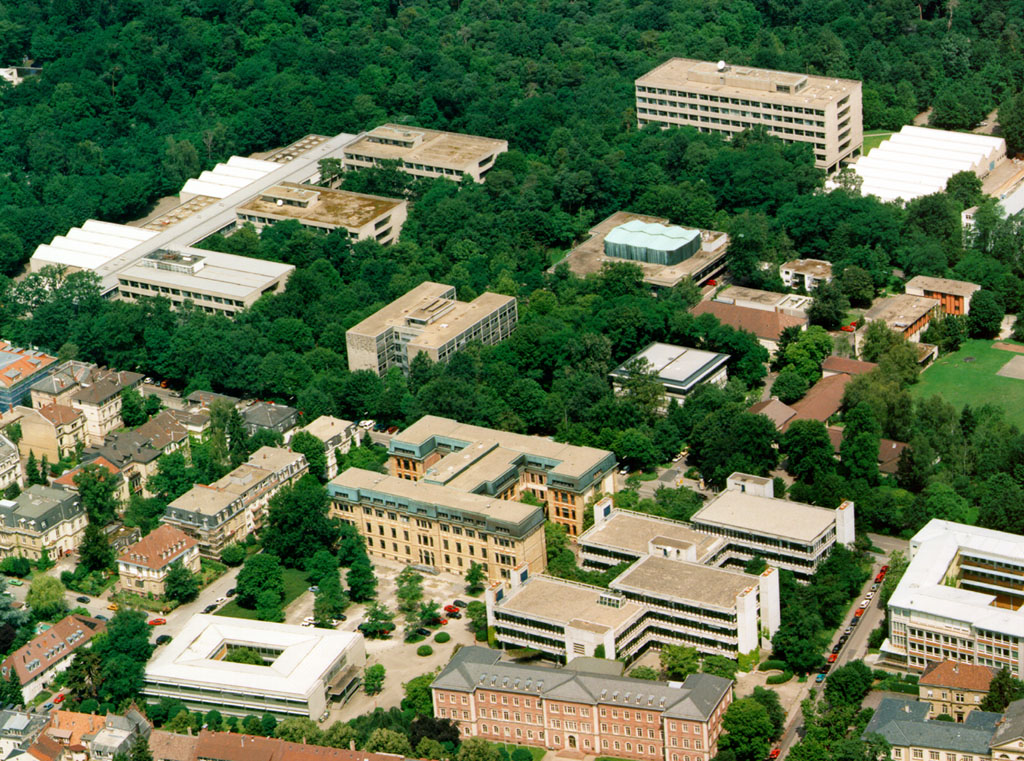
\includegraphics[width=0.5\textwidth]{060_Bilder/luftbild.jpg}
              \caption
              [Text des Luftbilds f�r das Abbildungsverzeichnis]              
              {\label{fig:bildJPEG}%
              Bild als JPEG}%
              \end{center}
              \end{figure}
             }

\fg{tbh}{060_Bilder/luftbild.jpg}{0.5\textwidth}{0}
        {Gleiches Bild mit Makro}
        {Gleiches Bild mit Makro gezeigt}

\fgB{060_Bilder/Kerbschlag.jpg}{!h}{0.6\textwidth}{0}%
    {Au�en: Eine l�ngere Bildunterschrift, die auch �ber mehrere Zeilen gehen kann}%
    {o}{Beside outer}

\fgB{060_Bilder/Kerbschlag.jpg}{!h}{0.4\textwidth}{0}%
    {Innen: Eine l�ngere Bildunterschrift, die auch �ber mehrere Zeilen gehen kann}%
    {i}{Beside inner}


\begin{figure}[]
              \begin{center}
              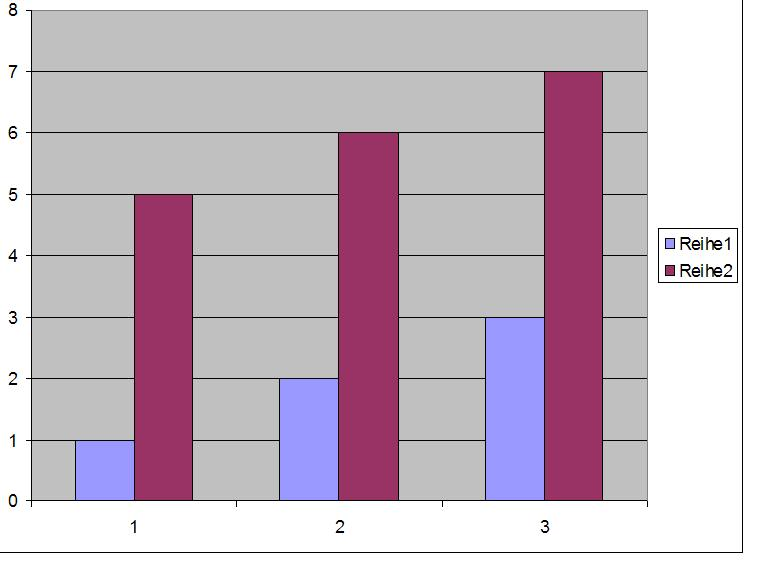
\includegraphics[width=0.8\textwidth]{060_Bilder/Excel-Paint.png}
              \caption%
              [Excel - Paint (copy and paste) save png]              
              {
              \label{fig:excelPaintpng}%
              Excel-Paint png
              }%
              \end{center}
              \end{figure}

\begin{figure}[]
              \begin{center}
              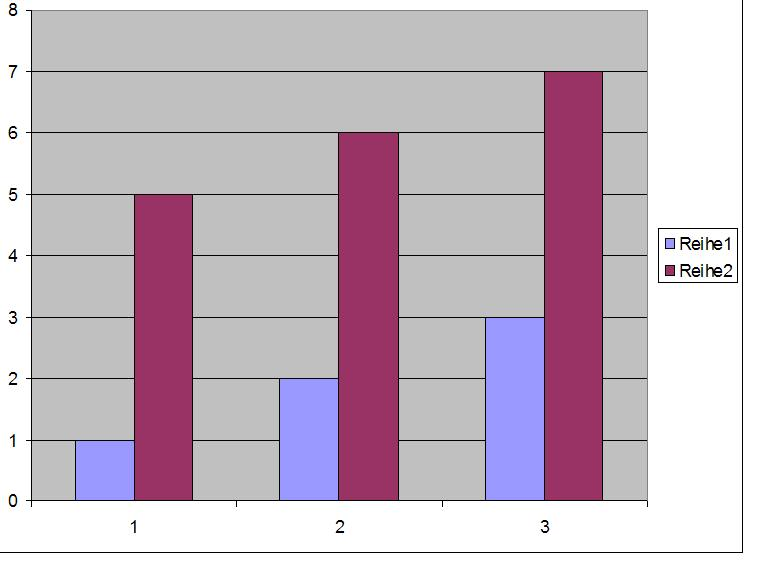
\includegraphics[width=0.8\textwidth]{060_Bilder/Excel-Paint.jpg}
              \caption
              [Excel - Paint (copy and paste) save jpg ]              
              {\label{fig:excelPaintjpg}%
              Excel-Paint jpg}%
              \end{center}
              \end{figure}

\begin{figure}[]
              \begin{center}
              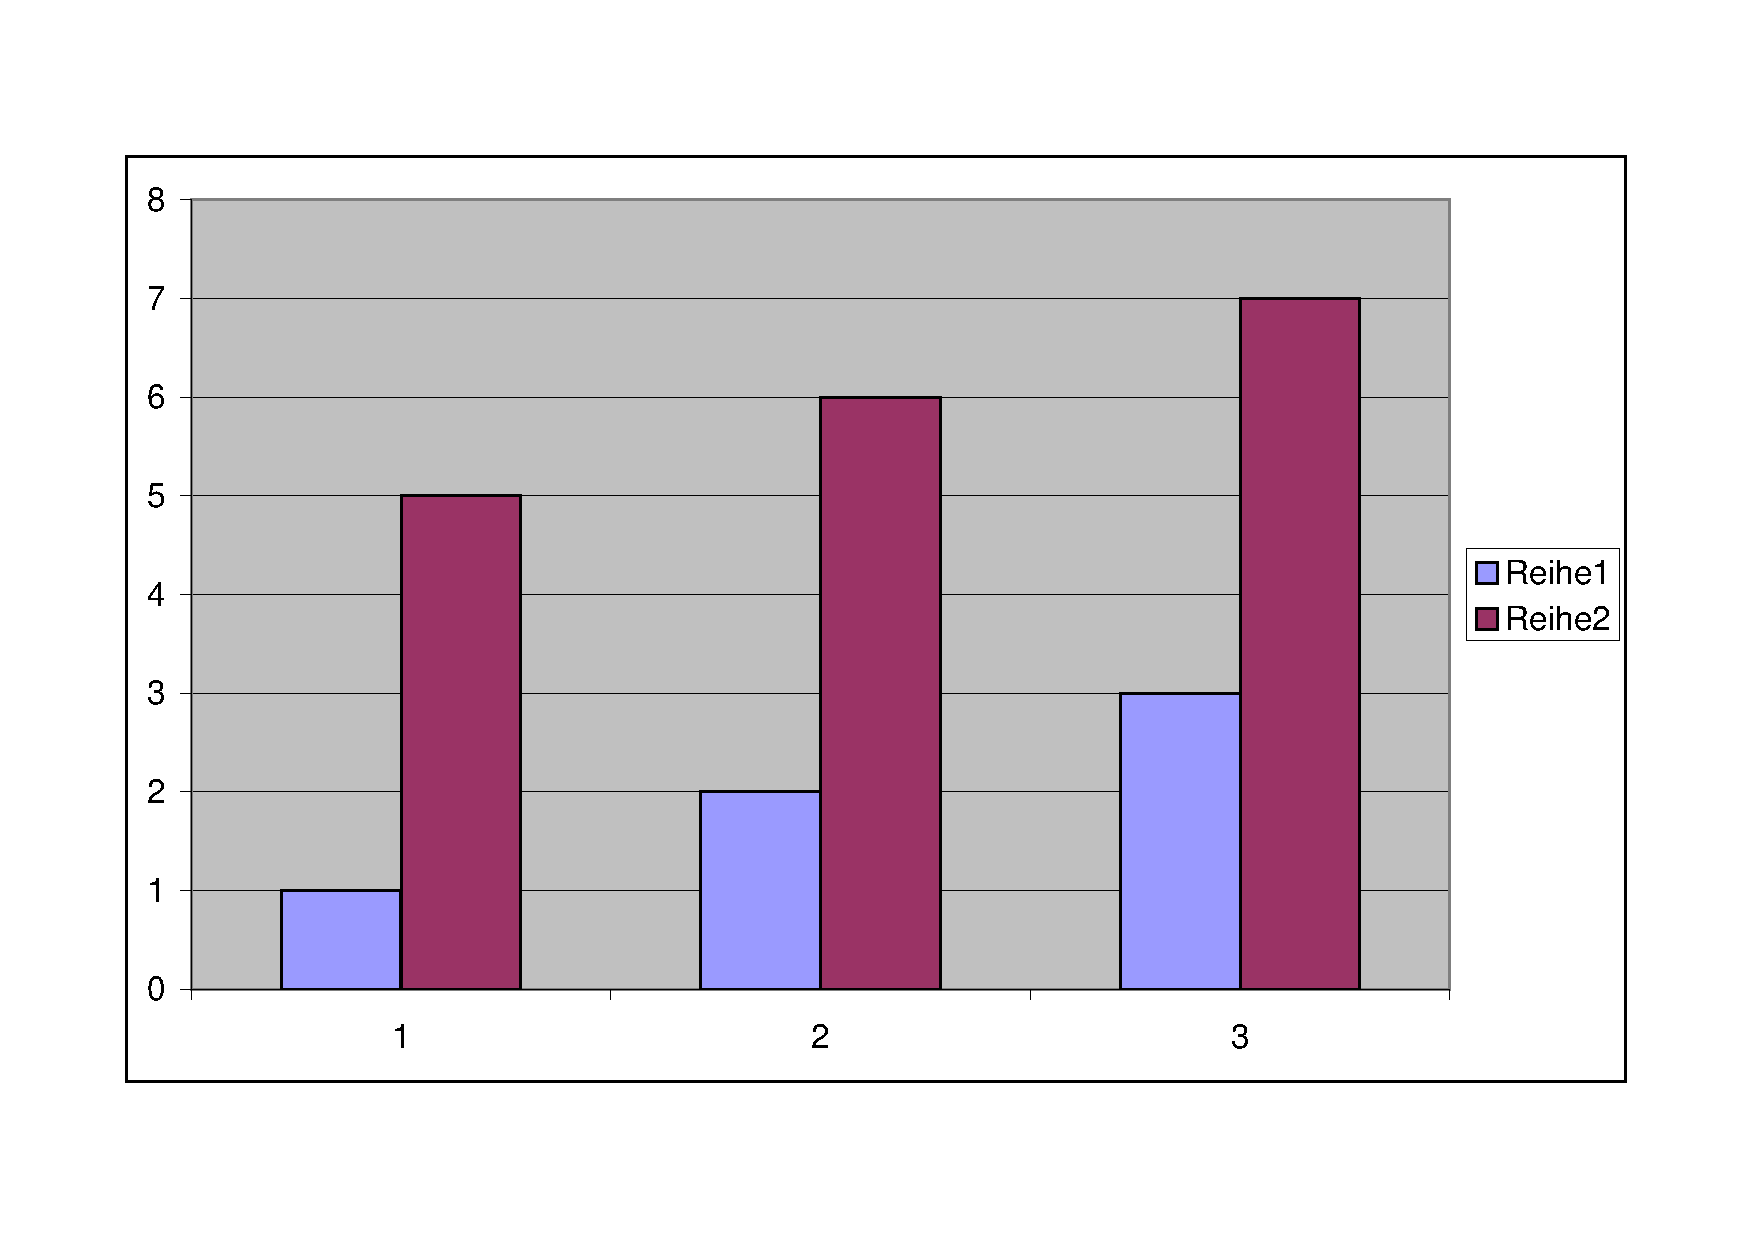
\includegraphics[width=0.8\textwidth]{060_Bilder/Excel-druck.pdf}
              \caption
              [Excel Druck pdf im AbbVerZeich]              
              {
              \label{fig:excelpdf}%
              Unterschrift Excel Druck pdf
              }%
              \end{center}
              \end{figure}
%                         
\clearpage
%   % DVI:ok?   PDF:ok   PS:niO  DVI->PS->PDF:niO   jpg:++ 
%                                              pdf: png:ok  
%%
%% Kapitel:
%%
%%======================================================================

\section{Bilder im pdf-Format}
\label{sec:Bilderpdf}


\emph{PDF} geht gut. Damit k�nnen elegant Zeichnungen
eingebunden werden, die \zB mit \emph{pstopdf} konvertiert sind.

\begin{figure}[h]
  \begin{center}
     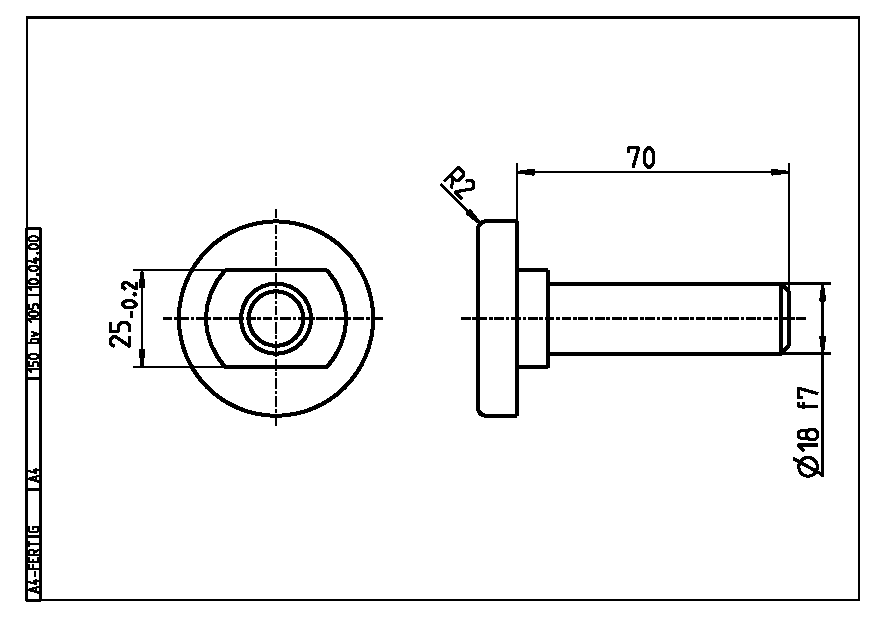
\includegraphics[width=0.8\textwidth]{%
              060_Bilder/bild1.pdf}
              \caption[Text zu Bild1 im Abb-Verzeischnis]{%
              \label{fig:bild1}
              Bild als PDF}
  \end{center}
\end{figure}

%
%
%\input{080_Macros/fuellung}
%
%

   % DVI:niO   PDF:ok   PS:niO  DVI->PS->PDF:niO   pdf:+ macht Problem
%%%
%% Kapitel:
%%
\chapter{Bilder mit PS}
\label{BilderPS}
%%======================================================================



\section{Bilder}

Etwas trickreich, da \LaTeX\ urspr�nglich daf�r nicht vorgesehen war.

\subsection{Postscript}
  
Die einfachste Variante benutzt \emph{Postscript}. Hat den Vorteil,
dass man CAD-Zeichnungen einfach einbinden kann. Beim Skalieren
werden die Strichbreiten auch skaliert. JPGs kann man mit
\texttt{jpeg2ps} in Postscript umwandeln.\\
Nachteil: Drucker muss Postscript k�nnen, \texttt{ghostscript} muss installiert sein!

{\begin{figure}[h]
              \begin{center}
              \epsfig{figure=0060/bild_ps.ps, width=100mm, angle=0}
              \caption{\label{fig:bild1ps} Postscriptbild} mit epsfig
              \end{center}
              \end{figure}
             }







    % DVI:niO  PDF:niO  PS:niO  DVI->PS->PDF:ok
%%%
%% Kapitel:
%%
\chapter{Bilder mit PS}
\label{BilderPS}
%%======================================================================



\section{Bilder}

Etwas trickreich, da \LaTeX\ urspr�nglich daf�r nicht vorgesehen war.

\subsection{Postscript}
  
Die einfachste Variante benutzt \emph{Postscript}. Hat den Vorteil,
dass man CAD-Zeichnungen einfach einbinden kann. Beim Skalieren
werden die Strichbreiten auch skaliert. JPGs kann man mit
\texttt{jpeg2ps} in Postscript umwandeln.\\
Nachteil: Drucker muss Postscript k�nnen, \texttt{ghostscript} muss installiert sein!

\includegraphics[width=80mm]{0060/bild_ps.ps} 	      
          







 % DVI:niO   PDF:niO  PS:niO  DVI->PS->PDF:niO
%%
%% Kapitel:
%%
\chapter{Mathematik}
\label{cha:Mathematik}
%%======================================================================

\section{Im Text}
%
Zuerst ein paar griechische Buchstaben: $\alpha$, $\beta$, $\tau$, $\pi$ $\xi$ $\psi$ $\Psi$.
%
Und was der Ingenieur mag: $\sigma\idx{zul}$, $W\idx{xy}$. 


\section{Abgesetzte Gleichungen}
%
Gleichungen werden automatisch mit Nummer, die auf das Kapitel enth�lt versehen:
\begin{equation}
\label{eqt:einstein}
E = mc^2
\end{equation}

Variablen werden immer automatisch kursiv gedruckt. Das e f�r die Eulersche Zahl muss 
daher in Gleichungen extra  mit  {\verb# \mathrm{e} #} \newline
als Nicht-Variable gekennzeichnet werden.

Nach DIN stehen Integralgrenzen  ober- bzw. unterhalb.\newline
Dazu wird der Befehl  {\verb# \int\limits_0^3 #} genutzt. Ein Beispiel gibt
\RefEq{eqt:integral}
\begin{equation}
\label{eqt:integral}
   \int\limits_0^3{x^2}dx=9 .
\end{equation}
%
Indizes werden im Allgemeinen nicht kursiv geschrieben, dazu verhilft ein
eigenes Makro {\verb+\newcommand{\idx}[1]{_\mathrm{#1}+}. Ein Beispiel
wird in \RefEq{eqt:bauer1} gegeben
\begin{equation}
  \label{eqt:bauer1}
   \dot{Q}\idx{Fl"ache} \sim \frac{1}{A\idx{Aussenwandfassade}}.
\end{equation}
%

Gleichungen ohne Nummern k�nnen mit mit \verb# \begin{displaymath} bzw. \end # erzeugt werden, 
alternativ mit \verb# \[ \] #
\begin{displaymath}
\sum_1^{\Xi} {\Psi}^2 = \frac{
          \int_{a_i^3}^{\sqrt{\omega - z^7}}
      }{
          \sqrt{\sqrt{e^{x^-3}}}
     }.
\end{displaymath}

%%
%% Kapitel:
%%
\chapter{Mathematik}
\label{cha:Mathematik}
%%======================================================================

\section{Im Text}
%
Zuerst ein paar griechische Buchstaben: $\alpha$, $\beta$, $\tau$, $\pi$ $\xi$ $\psi$ $\Psi$.
%
Und was der Ingenieur mag: $\sigma\idx{zul}$, $W\idx{xy}$. 


\section{Abgesetzte Gleichungen}
%
Gleichungen werden automatisch mit Nummer, die auf das Kapitel enth�lt versehen:
\begin{equation}
\label{eqt:einstein}
E = mc^2
\end{equation}

Variablen werden immer automatisch kursiv gedruckt. Das e f�r die Eulersche Zahl muss 
daher in Gleichungen extra  mit  {\verb# \mathrm{e} #} \newline
als Nicht-Variable gekennzeichnet werden.

Nach DIN stehen Integralgrenzen  ober- bzw. unterhalb.\newline
Dazu wird der Befehl  {\verb# \int\limits_0^3 #} genutzt. Ein Beispiel gibt
\RefEq{eqt:integral}
\begin{equation}
\label{eqt:integral}
   \int\limits_0^3{x^2}dx=9 .
\end{equation}
%
Indizes werden im Allgemeinen nicht kursiv geschrieben, dazu verhilft ein
eigenes Makro {\verb+\newcommand{\idx}[1]{_\mathrm{#1}+}. Ein Beispiel
wird in \RefEq{eqt:bauer1} gegeben
\begin{equation}
  \label{eqt:bauer1}
   \dot{Q}\idx{Fl"ache} \sim \frac{1}{A\idx{Aussenwandfassade}}.
\end{equation}
%

Gleichungen ohne Nummern k�nnen mit mit \verb# \begin{displaymath} bzw. \end # erzeugt werden, 
alternativ mit \verb# \[ \] #
\begin{displaymath}
\sum_1^{\Xi} {\Psi}^2 = \frac{
          \int_{a_i^3}^{\sqrt{\omega - z^7}}
      }{
          \sqrt{\sqrt{e^{x^-3}}}
     }.
\end{displaymath}

%-------------------------------------------------------------------
% Literaturliste
%-------------------------------------------------------------------
%-----------------------------------------------------------
% Literaturliste
%-----------------------------------------------------------
% Format der Eintraege:
%   \lit{NAME DES EINTRAGS}{VERFASSER}{TITEL}{AUFLAGE}
% Hinweise:
%   \lit ist ein Makro, das in macro.tex definiert ist.
%   Es bastelt aus den 4 Uebergabeparametern das richtige
%   Format fuer bibtex zusammen. Damit ist man bei der 
%   Formatierung der Literaturliste freier, da sie nur
%   an einer Stelle geaendert werden muss. Zeilenumbrueche
%   am Ende der Eingabeparameter werden automatisch 
%   eingefuegt. Soll ein Parameter ueber mehere Zeilen
%   gehen, so muss der Umbruch im Parameter uebergeben
%   werden.
%
%   Zitiert wird mit \cite{NAME_DES_EINTRAGS}
%
%   Die Eintraege selber werden in der Reihenfolge, in
%   der sie in dieser Datei stehen nummeriert.
%-----------------------------------------------------------

% literatur.tex enthaelt nur Eintraege, Header und Footer stehen hier,
% damit literatur.tex sortiert werden kann!
%

Dieses Verzeichnis ist noch NICHT nach DIN.

\begin{thebibliography}{15}
       % Die folgende Zeile erzwingt einen Eintag ins Inhaltsverz.
       \addcontentsline{toc}{section}{Literatur} 
       \label{cha:LitVerzeichnis}
%===========================================================

\lit{din1505}{NORM DIN 1505-2 Ausgabe 1984-01}
               {Titelangaben von Dokumenten; Zitierregeln,}
						   {Beuth-Verlag, 2006}

\lit{din5008}{NORM DIN 5008 Ausgabe 2005-05}
              {Schreib- und Gestaltungsregeln f�r die Textverarbeitung,}
              {Beuth-Verlag, 2006}

\lit{din5008web}{NORM DIN 5008 Ausgabe 2005-05}
              {Schreib- und Gestaltungsregeln f�r die Textverarbeitung,}
              {http://www.din5008.de/p0400010.htm, Stand 23.09.2006}
				  
\lit{Einstein}{Einstein, Albert}
              {Komische Gleichungen}
              {Relativverlag, 1921}

\lit{komabook}{Kohm, Markus; Morawski, Jens-Uwe}
							{\KOMAScript{} eine Sammlung von Klassen und Paketen f�r {\LaTeX2e}}
							{Lehmans Fachbuchhandlung, ISBN 3-86541-089-8, Januar 2006}

\lit{komaweb}{\KOMAScript{} Documentation project}
	            {\href{http://koma-script.net.tf}{http://koma-script.net.tf},}
	            {Sep. 2006} 
\lit{DIN22}	  {DIN-Taschenbuch 22 Ausgabe 1999-03}
              {Einheiten und Begriffe f�r physikalische Gr��en}
              {Beuth-Verlag, 2006} % 98 Euro
\lit{DIN202}	{DIN-Taschenbuch 202 Ausgabe 1994-07}
              {Formelzeichen, Formelsatz, Mathematische Zeichen und Begriffe}
              {Beuth-Verlag, 2006}% 81 Euro   
%\lit{DIN461}	{NORM DIN 461 Ausgabe 1973-03}
%              {Graphische Darstellung in Koordinatensystemen}
%              {Beuth-Verlag, 2006}% 40 Euro   


%===========================================================
\end{thebibliography}
       %Pfad zur Datei
%
%  siehe bibtex und packages
%
% gerabbrv, geralpha, gerapali, gerplain, gerunsrt, din1505
\bibliographystyle{gerplain}
%
% abbrvdin, alphadin, ndatdin, plaindin, usrtdin
%\bibliographstyle{plaindin}
%
\bibliography{listen/literatur}  % bib datei

       \addcontentsline{toc}{section}{Literatur}             %Pfad zur Datei
%-------------------------------------------------------------------
% Index
%-------------------------------------------------------------------
\printindex
%-------------------------------------------------------------------
\newpage
%-------------------------------------------------------------------
% Anhang
%-------------------------------------------------------------------
\appendix        % Alles was hier kommt, landet im Anhang
%-------------------------------------------------------------------
%%
%  Kontakt-Daten
%==============================================================================
\chapter{Anhang}

\section{Bildanhang}
%\newpage
%------------------------------------------------------------------------------
% - - - - - - - - - - - - - - - - - - - - - 
\begin{figure}[!h]
   \begin{center}
   \fbox{
      \includegraphics[width=0.95\textwidth,angle=0]% Achtung pdf muss schon Hochkant sein !
      {anhang/KontaktDaten.pdf}
      }
      \caption{\label{fig:KontaktDaten}
               Wichtige Namen, Anschriften und Telefonnummnern}
   \end{center}
 \end{figure}
 
\clearpage

%------------------------------------------------------------------------------
%\section{Zeit- und Arbeitsplan}
%\label{sec:BeispielPlan}
% - - - - - - - - - - - - - - - - - - - - - 
\begin{figure}[!h]
   \begin{center}
   \fbox{
      \includegraphics[width=0.95\textwidth,angle=0]% Achtung pdf muss schon Hochkant sein !
      {anhang/BspTerminplan.pdf}
      }
      \caption{\label{fig:BspPlan}
               Beispiel f�r Zeit- und Arbeitsplan}
   \end{center}
 \end{figure}
 
\clearpage
% - - - - - - - - - - - - - - - - - - - - - 
 \begin{figure}[!h]
   \begin{center}
   \fbox{
      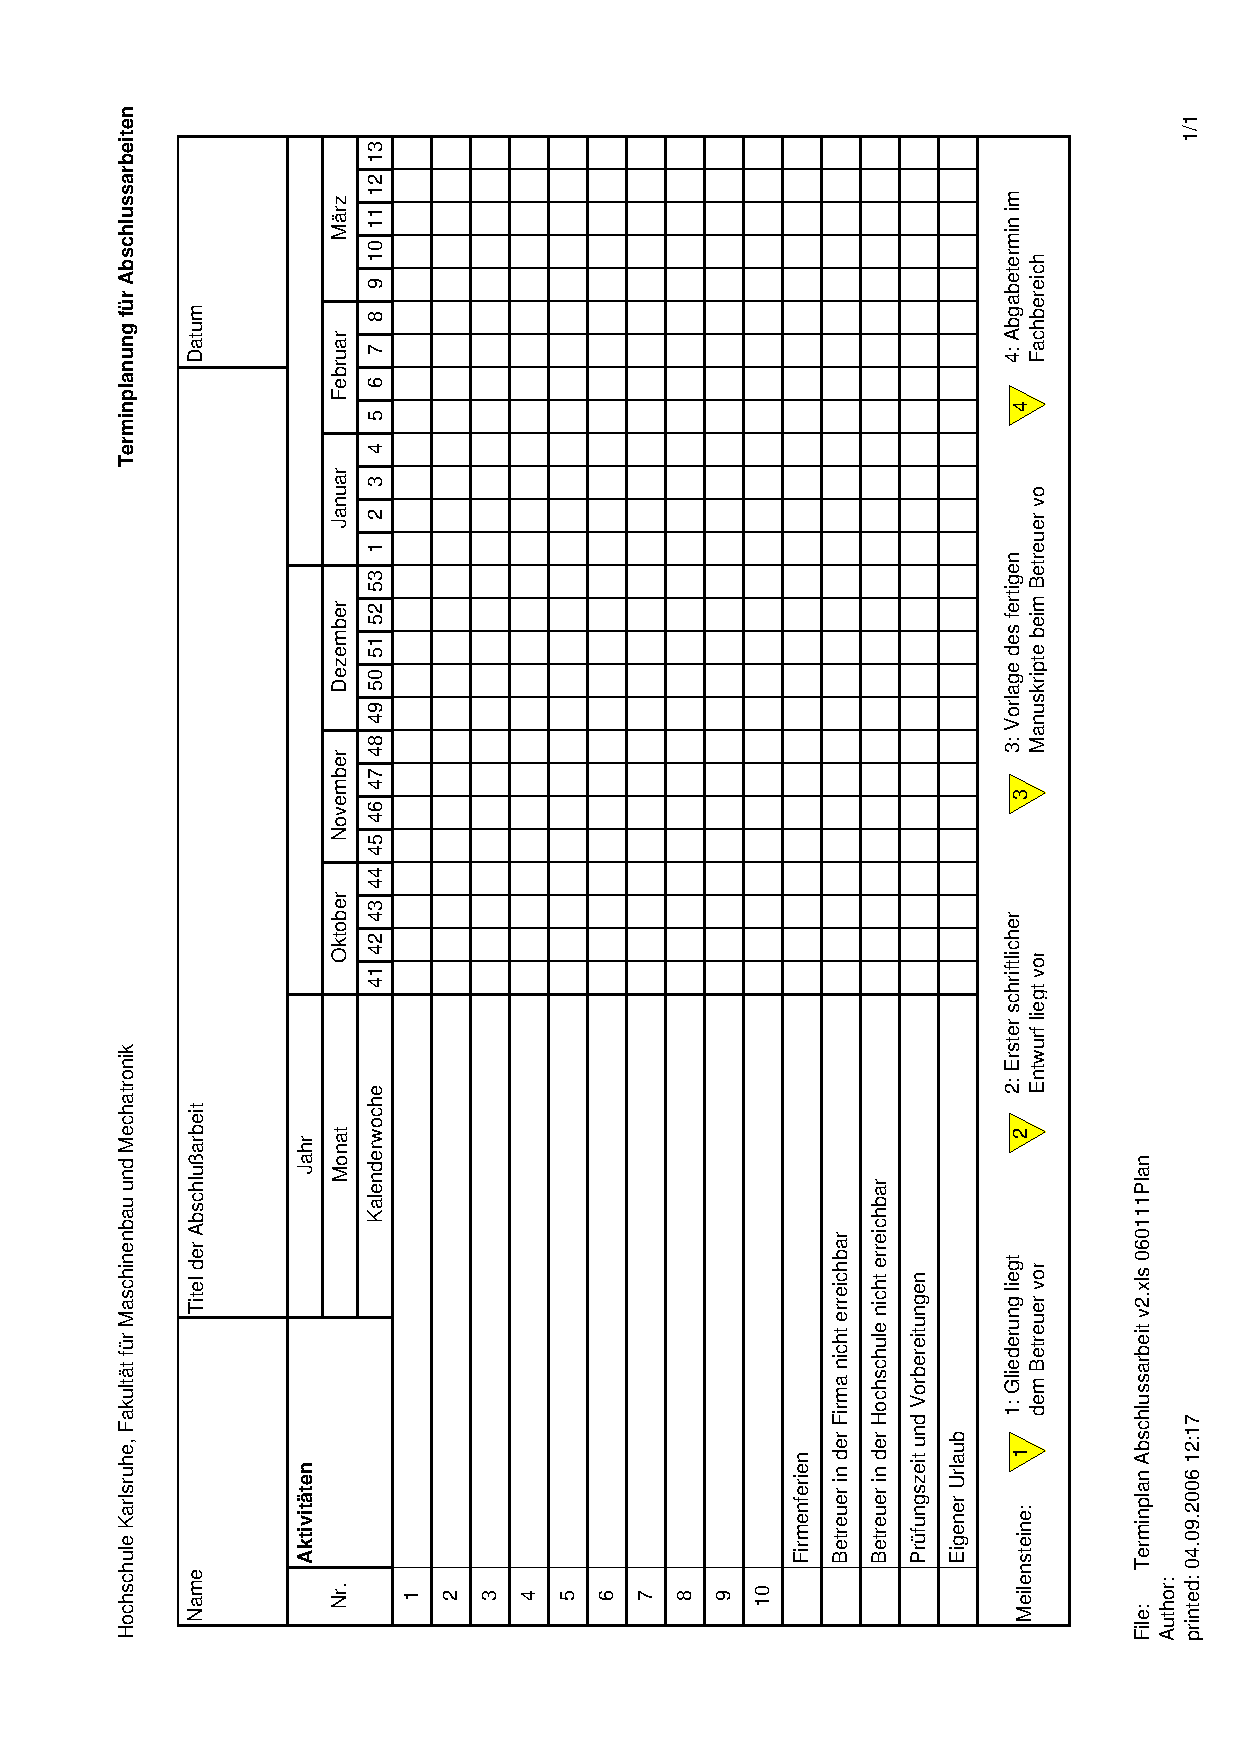
\includegraphics[width=0.95\textwidth,angle=0]
      {anhang/Terminplan_Abschlussarbeit_v2.pdf}
      }
      \caption{\label{fig:Plan}
               Vorlage f�r Zeit- und Arbeitsplan}
   \end{center}
 \end{figure}

\clearpage

%------------------------------------------------------------------------------
%\section{Titelseite}
%\label{sec:Titelseite}
% - - - - - - - - - - - - - - - - - - - - - 
 \begin{figure}[!h]
   \begin{center}
   \fbox{
      \includegraphics[width=0.95\textwidth, angle=0]{anhang/Titelseite}
      }
      \caption{\label{fig:Titelseite}
               Muster f�r die Titelseite}
   \end{center}
 \end{figure}

\clearpage

%------------------------------------------------------------------------------
%\section{Deckblatt}
%\label{sec:Deckblatt}

% - - - - - - - - - - - - - - - - - - - - - 
 \begin{figure}[!h]
   \begin{center}
   \fbox{
      \includegraphics[width=0.95\textwidth, angle=0]{anhang/Deckblatt}
        }     
      \caption{\label{fig:Deckblatt}
               Muster f�r das Deckblatt}
   \end{center}
 \end{figure}
 
 \clearpage
 
%------------------------------------------------------------------------------
%\section{Erkl�rung und Sperrvermerk}
%\label{sec:Erklaerung}
 
% - - - - - - - - - - - - - - - - - - - - -  
 \begin{figure}[!h]
   \begin{center}
   \fbox{
      \includegraphics[width=0.95\textwidth, angle=0]{anhang/Erkl�rung_Sperrvermerk}
        }     
      \caption{\label{fig:Erklaerung}
               Erkl�rung und Beispiel f�r Sperrvermerk}
   \end{center}
 \end{figure}
 
 \clearpage
 
%------------------------------------------------------------------------------
%\section{Inhaltsverzeichnis}
%\label{sec:Inhaltsverzeichnis}
 
% - - - - - - - - - - - - - - - - - - - - -  
 \begin{figure}[!h]
   \begin{center}
   \fbox{
      \includegraphics[width=0.95\textwidth, angle=0]{anhang/BspInhaltsverzeichnis}
        }     
      \caption{\label{fig:BspInhaltsverzeichnis}
               Beispiel f�r eine Inhaltsverzeichnis}
   \end{center}
 \end{figure}
 
 \clearpage
 
%------------------------------------------------------------------------------
%\section{Zusammenfassung}
%\label{sec:Zusammenfassung}
 
% - - - - - - - - - - - - - - - - - - - - -  
 \begin{figure}[!h]
   \begin{center}
   \fbox{
      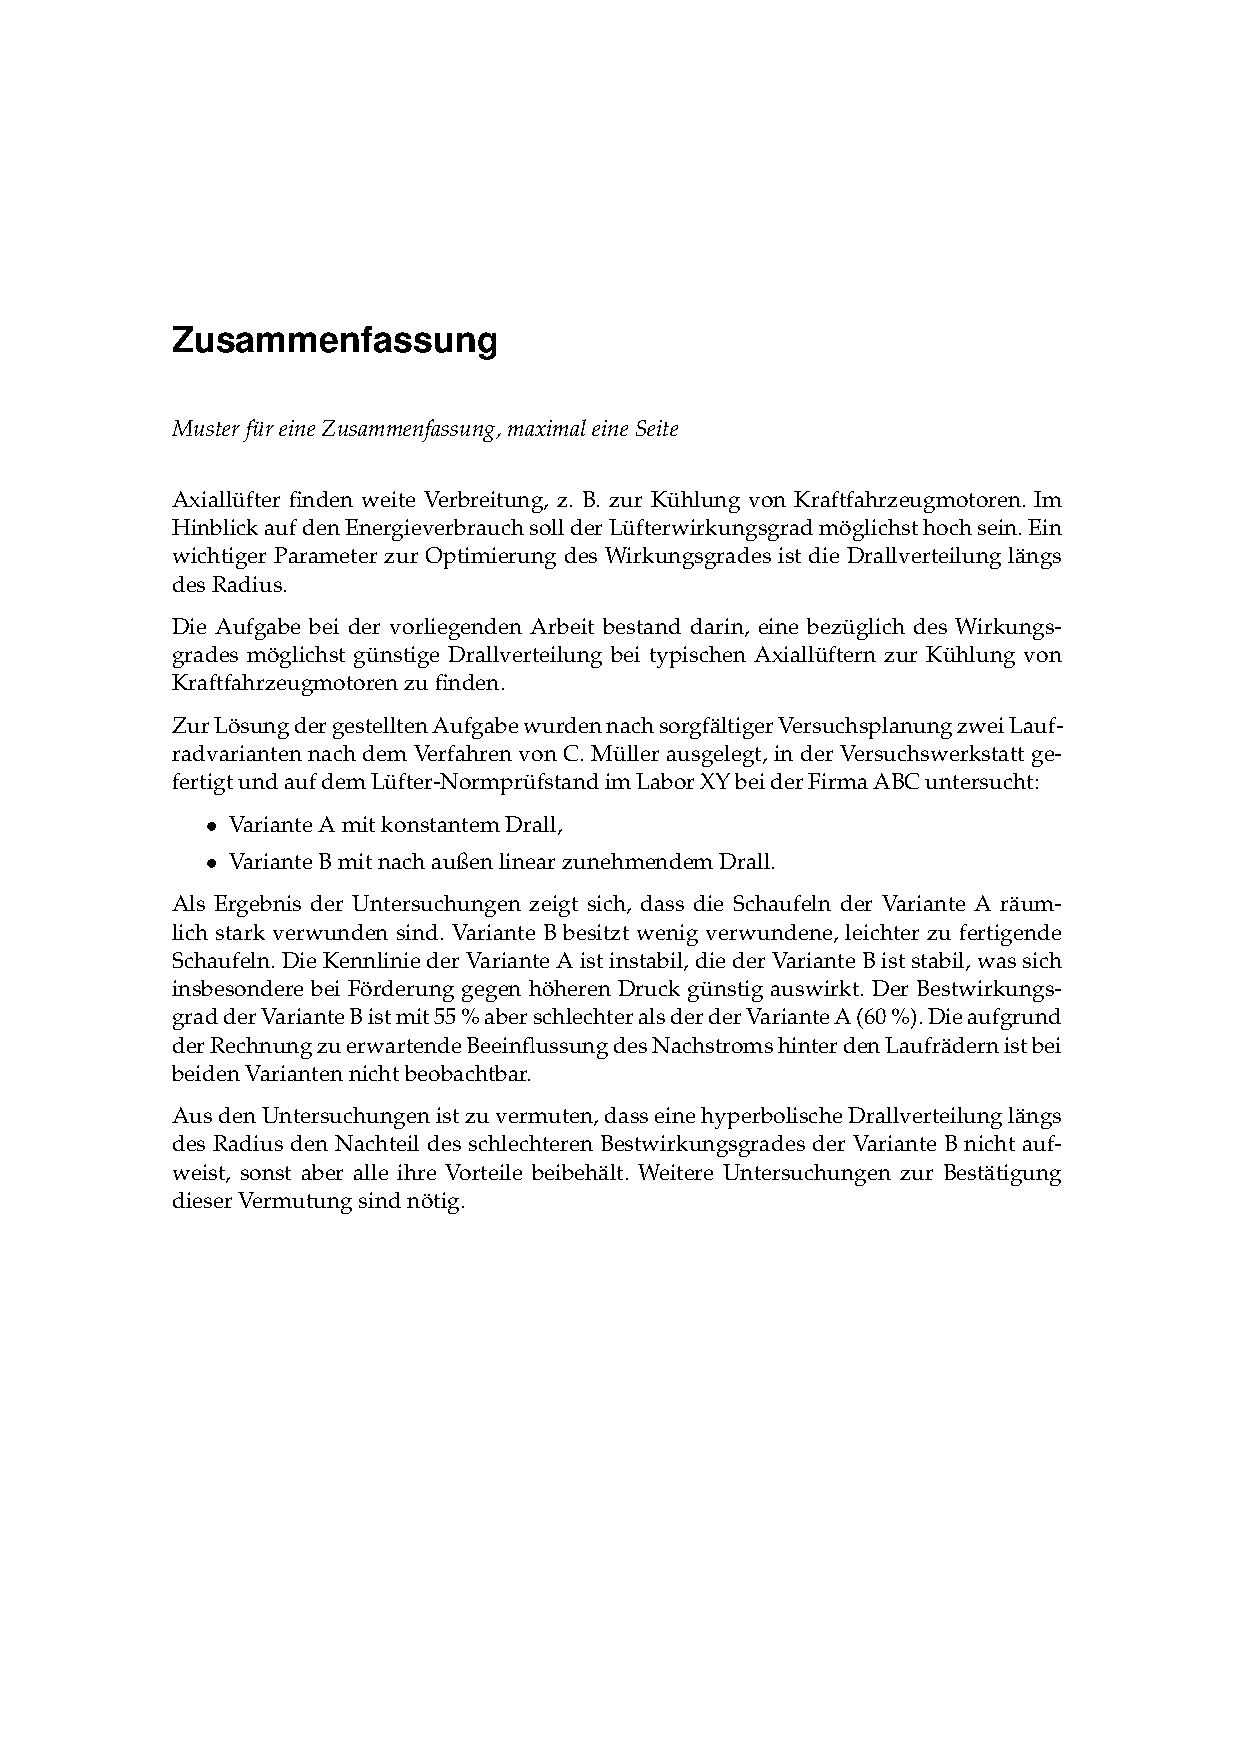
\includegraphics[width=0.95\textwidth, angle=0]{anhang/BspZusammenfassung}
        }     
      \caption{\label{fig:BspZusammenfassung}
               Beispiel f�r eine Zusammenfassung}
   \end{center}
 \end{figure}
 
 \clearpage
 
%------------------------------------------------------------------------------ 
%\section{Literaturverzeichnis}
%\label{sec:Literaturverzeichnis}
 
% - - - - - - - - - - - - - - - - - - - - -  
%\begin{figure}[!h]
%   \begin{center}
%   \fbox{
%      \includegraphics[width=0.95\textwidth, angle=0]{anhang/BspLitVerzeichnis}
%        }     
%      \caption{\label{fig:BspLitVerzeichnis}
%               Beispiel f�r ein Literaturverzeichnis}
%   \end{center}
% \end{figure}
% 
% \clearpage
%------------------------------------------------------------------------------   

% - - - - - - - - - - - - - - - - - - - - -  
 \begin{figure}[!h]
   \begin{center}
   \fbox{
      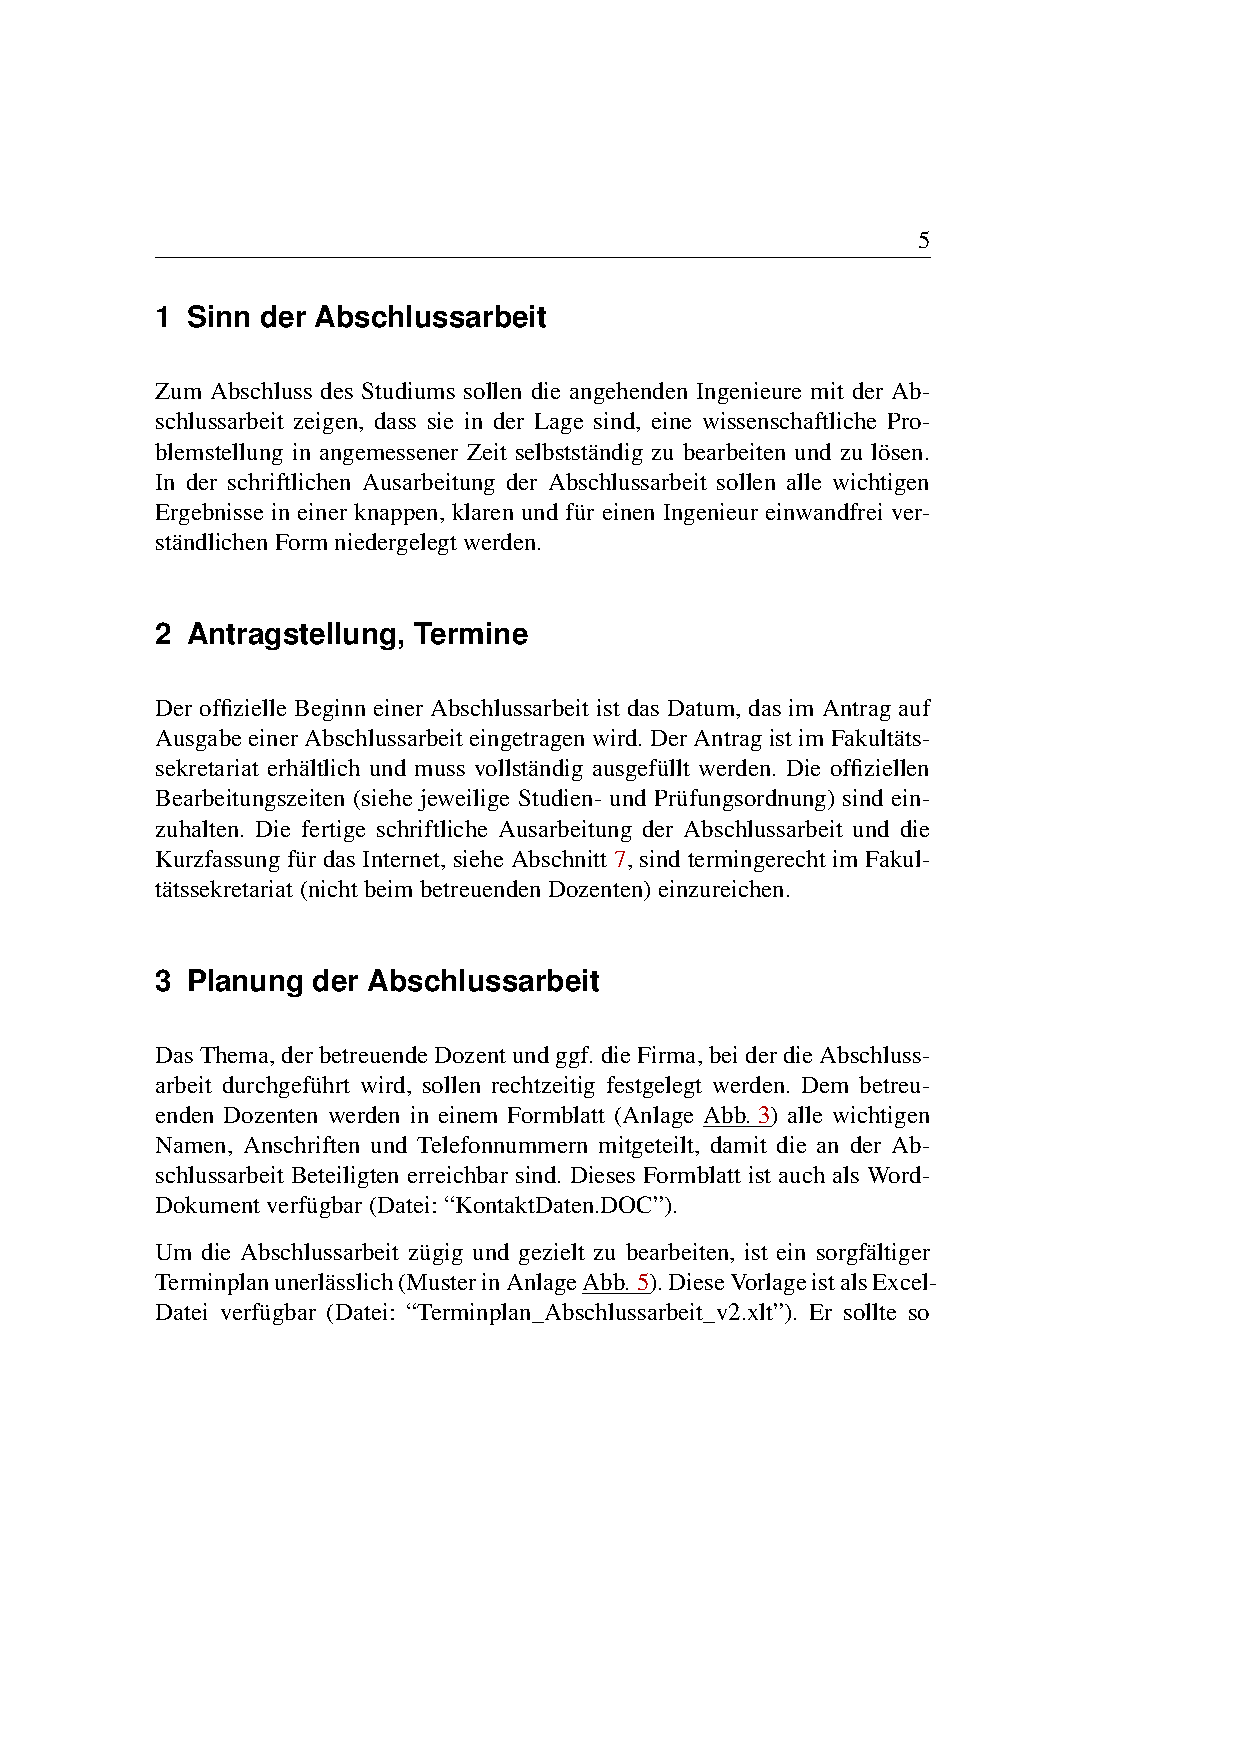
\includegraphics[width=0.95\textwidth, angle=0]{anhang/BspTimes12}
        }     
      \caption{\label{fig:BspTimes12}
               Beispiel--Satz mit Times 12 pt}
   \end{center}
 \end{figure}
 
 \clearpage
%------------------------------------------------------------------------------   

% - - - - - - - - - - - - - - - - - - - - -  
 \begin{figure}[!h]
   \begin{center}
   \fbox{
      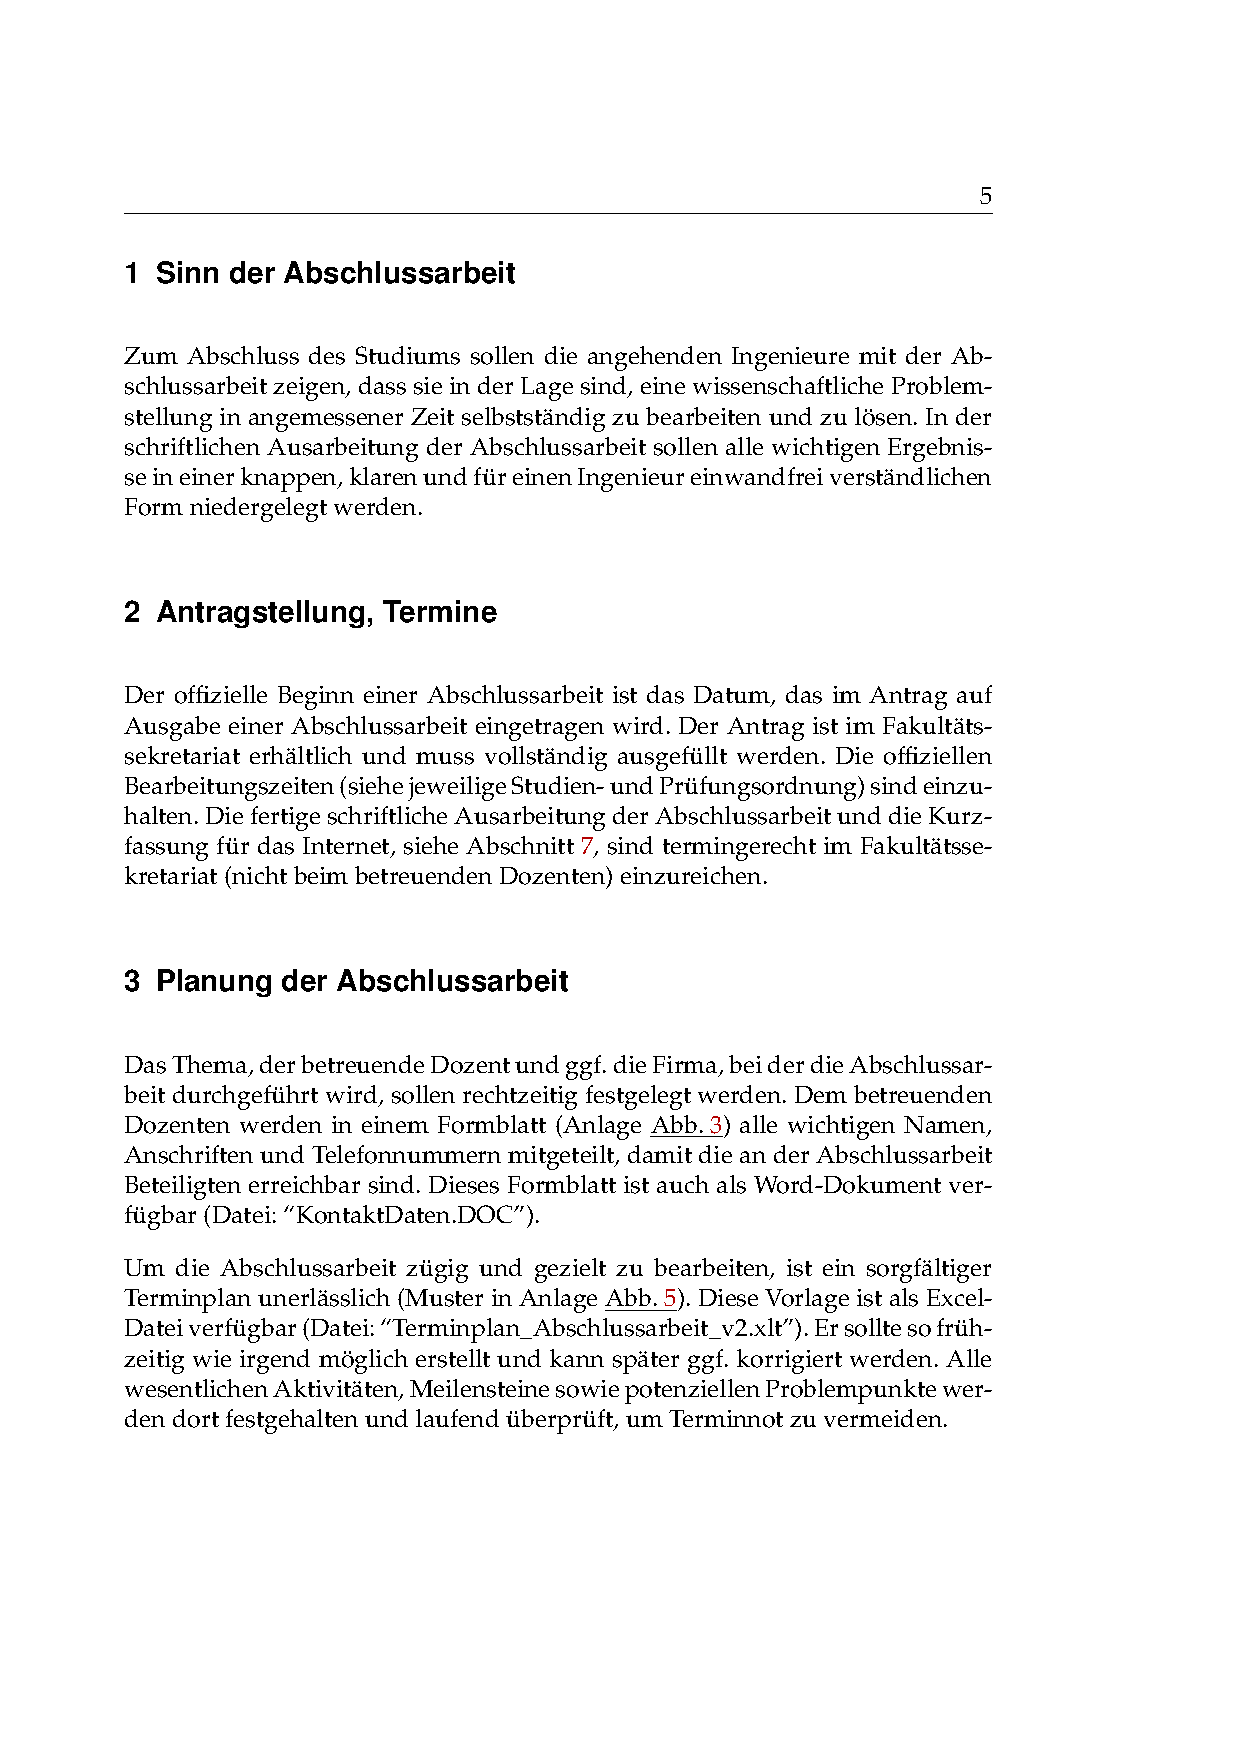
\includegraphics[width=0.95\textwidth, angle=0]{anhang/BspPalatino12}
        }     
      \caption{\label{fig:BspPalatino12}
               Beispiel--Satz mit Palatino 12 pt}
   \end{center}
 \end{figure}
 
 \clearpage
%------------------------------------------------------------------------------   
% - - - - - - - - - - - - - - - - - - - - -  
 \begin{figure}[!h]
   \begin{center}
   \fbox{
      \includegraphics[width=0.95\textwidth, angle=0]{anhang/BspPalatino11}
        }     
      \caption{\label{fig:BspPalatino11}
               Beispiel--Satz mit Palatino 11 pt}
   \end{center}
 \end{figure}
 
 \clearpage
%------------------------------------------------------------------------------   
% - - - - - - - - - - - - - - - - - - - - -  
 \begin{figure}[!h]
   \begin{center}
   \fbox{
      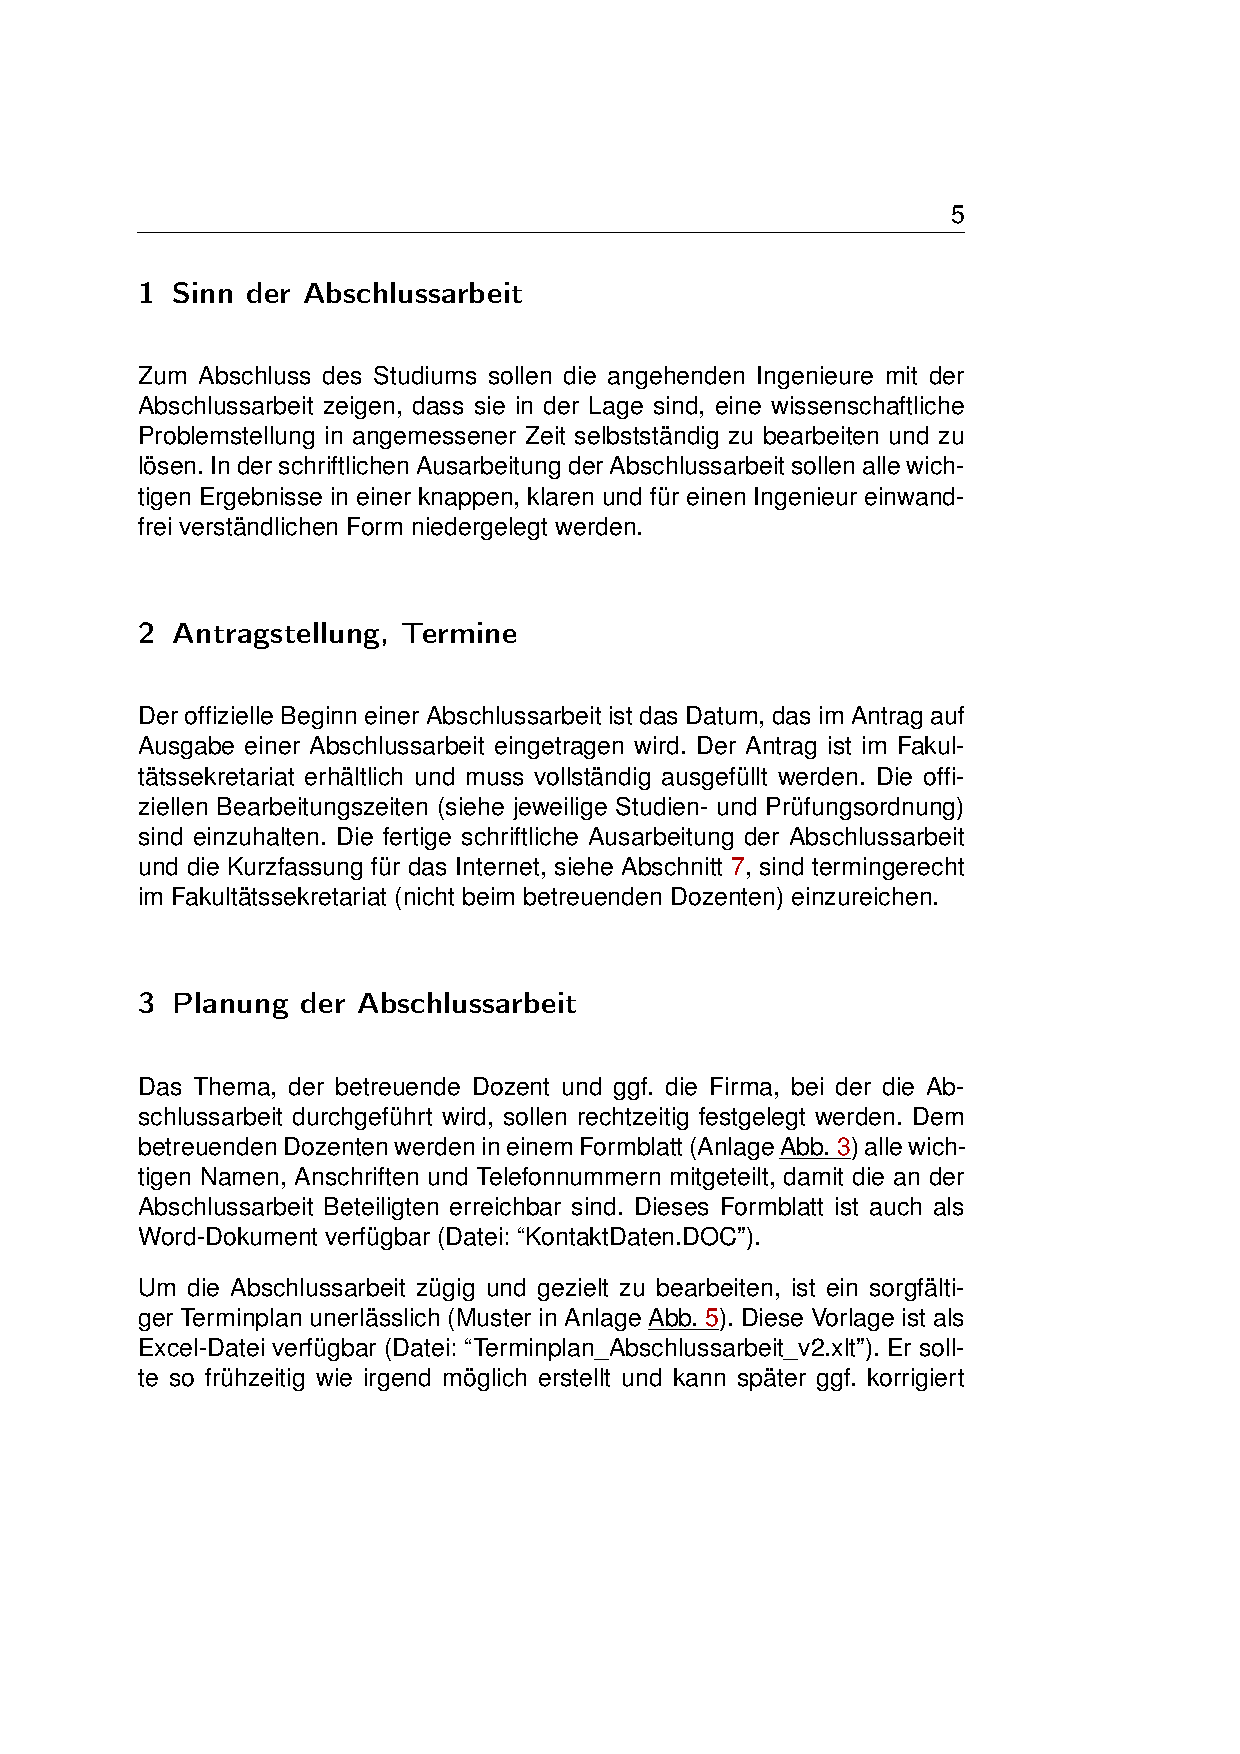
\includegraphics[width=0.95\textwidth, angle=0]{anhang/BspHelvetica12}
        }     
      \caption{\label{fig:BspHevetica12}
               Beispiel--Satz mit Helvetica 12 pt}
   \end{center}
 \end{figure}
 
 \clearpage
%------------------------------------------------------------------------------   




\chapter{Komplizierte Sch�tzer-Begriffe endlich in Deutsch} 

Den meisten von uns ist klar, da� das englische Wort Computer vom Verb compute (rechnen, sch�tzen) kommt, da� ein Computer also ein Rechner oder Sch�tzer ist. Aber noch immer gibt es viele Zeitgenossen, die vielleicht gerade erst anfangen, sich mit diesem komplexen Thema etwas n�her zu befassen. Dieser Artikel soll all jenen helfen, die nicht mit einem Spielbuben aufgewachsen sind und die nicht schon von Kind auf all diese verwirrenden Begriffe wie eine Muttersprache auf nat�rlichem Wege erlernen konnten. 

\section{Mutterbrett und Riesenbiss} 
Beginnen wir vielleicht mit den einfachen Dingen, die wir sehen, anfassen und damit auch noch begreifen k�nnen! 
Alle Bausteine eines Sch�tzers werden als Hartware bezeichnet. Es ist sehr wichtig, bei der Auswahl der Hartware sorgsam zu sein, denn nur auf guter Hartware kann die Weichware richtig schnell laufen. 
Bei der Hartware ist das Mutterbrett von besonderer Bedeutung. Das Mutterbrett soll unter anderem mit einem Schnittsatz von Intel ausger�stet sein. Die gleiche Firma sollte auch die ZVE (Zentrale Voranschreitungs-Einheit) geliefert haben. Damit wir uns bei der Arbeit richtig wohl f�hlen, sollten wir einen 17-Daumenlang-Vorzeiger oder eine 15-Daumenlang-Fl�ssig-Kristall-Schaustellung verwenden. Zum Zwecke der Augenschonung sollten Sie den Vorzeiger oder die Schaustellung auf mindestens 70 Bildern pro Sekunde Erholungsgeschwindigkeit und wahre Farbe einstellen. Ein ordentliches Schl�sselbrett darf auch nicht fehlen. Damit anspruchsvolle Weichware eine gute Vorf�hrung zeigt, m�ssen mindestens 64 Riesenbiss Erinnerung eingebaut sein. Nat�rlich geh�rt neben dem 3 l/2-Zoll-Schlappscheibentreiber auch eine Dichtscheiben-Lese-nur- Erinnerung zur Grundausr�stung. Eine Hartscheibe mit 10 Gigantischbiss d�rfte f�r die n�chsten zwei bis drei Jahre ausreichend Erinnerungsplatz f�r Weichware und Daten bieten. Wenn wir unseren PS (pers�nlichen Sch�tzer) auch zum Spielen, benutzen wollen, sollten wir uns neben der Maus auch noch einen Freudenstock und ein gutes Schallbrett anschaffen.


\section{Winzigweich und Kraftpunkt} 
So, hierdurch sind nun die optimalen Grundlagen f�r Einbau und Betrieb der Weichware geschaffen! Damit die Weichware auf unserer Hartware �berhaupt laufen kann, braucht es ein Betriebssystem. Es empfiehlt sich heute, ein solches mit einem grafischen Benutzer-Zwischengesicht zu installieren. Besonders weit verbreitet sind die Systeme Winzigweich-Fenster 95 und das neuere Fenster 98 des gleichen Herstellers mit integriertem Zwischennetz- Erforscher. Letzteres ist �rgerlich f�r Leute, die lieber mit dem Netzschaft-Schiffs\-f�hr\-er\-wel\-lenreiten arbeiten wollen. Winzigweich-Systeme haben die Eigenart, �fter mal einen Krach zu verursachen. Dann m�ssen sie neu gestiefelt werden. 
Schlager verzichten auf ein grafisches Zwischengesicht und bevorzugen ein altes, Befehlslinien-Ausdeuter- ausgerichtetes Vielfachbeaufgabungs-Betriebssystem namens Einheitlix, weil sie behaupten, sie w��ten schon, was sie tun. Einheitlix hat den Vorteil, da� es auf verschiedenen Sch�tzern mit unterschiedlichen ZVEs l�uft. Auch auf �lteren Ger�ten hat es eine gute Vorf�hrung. Einheitlix ist furchtbar umst�ndlich zu bedienen, aber der Schl�ger kann damit alles machen, was er will. Zum Beispiel ganz schnell den Sch�tzer kaputt. 
F�r Leute, die mit ihrem Sch�tzer anspruchsvolle Arbeiten erledigen wollen, gibt es unter Fenster 95/98 das ber�hmte ''B�ro fachm�nnisch 97'' bzw. ''B�ro fachm�nnisch 2000''. Dieses Erzeugnis besteht aus den neuesten Ausgaben der WeichwarenWort, �bertreff, Kraftpunkt und Zugriff. Damit stehen dem Benutzer alle wichtigen Funktionen wie Wortveredelung,Ausbreitblatt, Pr�sentationsgrafik und Datenst�tzpunkt-Behandlung zur Verf�gung. Viel billiger ist das Sternen-B�ro von der Hamburger Firma Sternen-Abteilung, das es auch f�r Einheitlix gibt. Sehr beliebt ist sind auch der Sumpfbl�ten-Organisierer und Schichtk�se-Ausdruck, das f�r Tischplatten-Ver�ffentlichung gebraucht wird.


\section{Aufsteller und Einsetzer} 
Wer selbst gerne Anwendungen entwickelt, kann dies unter Fenster beispielsweise mit dem modernen Sichtbar Grundlegend tun. Nat�rlich gibt es vor dem Gebrauch auch gewisse Hindernisse zu �berwinden. Die Weichware mu� zuerst via Aufsteller oder Einsetzer auf der Hartscheibe eingerichtet werden. Das kann sehr viel Zeit brauchen, wenn sie urspr�nglich auf Schlappscheiben geliefert wurde. Das Einrichten mit einer Dichtscheiben-Lese-nur-Erinnerung ist sehr viel angenehmer und schneller. Leider stellen aber auch hier die Aufsteller oft Fragen, die von vielen unverst�ndlichen Begriffen nur so wimmeln. Aber die wollen wir uns ein andermal vornehmen ...

\chapter{�bersetzungshilfe}  

\begin{tabbing}
\hspace{85mm} \= \\

17-Daumenlang-Vorzeiger \> 17'' Monitor  \\
15-Daumenlang-Fl�ssig-Kristall-Schaustellung \> 15'' LC-Display  \\
Aufsteller \> Setup  \\
Ausbreitblatt \> Spreadsheet  \\
Befehlslinien-Ausdeuter \> Command Line Interpreter  \\
B�ro fachm�nnisch 97 \> Office 97  \\
Datenst�tzpunkt \> Database = \\
Dichtscheiben-Lese-nur-Erinnerung \> Compact Disc Read Only Memory  \\
Einheitlix \> Unix  \\
Einsetzer \> Install  \\
Erholungsgeschwindigkeit \> Refresh Rate  \\
Erinnerung \> Memory  \\
Fenster \> Windows  \\
Freudenstock \> Joystick  \\
gestiefelt \> gebooted  \\
Gigantischbiss \> Gigabyte  \\
Hartscheibe \> Harddisk  \\
Hartware \> Hardware  \\
Krach \> Crash  \\
Kraftpunkt \> PowerPoint  \\
Mutterbrett \> Motherboard  \\
Netzschaft-Schiffsf�hrer \> Netscape Navigator  \\
Riesenbiss \> Megabyte  \\
Schallbrett \> Sound Card  \\
Sch�tzer \> Computer  \\
Schichtk�se- Ausdruck \> Quark Xpress  \\
Schlager \> Hacker  \\
Schlappscheiben \> Floppy  \\
Schlappscheibentreiber \> Floppy Drive  \\
Schl�sselbrett \> Keyboard  \\
Schnittsatz \> Chipsatz  \\
Sichtbar Grundlegend \> Visual Basic  \\
Spielbuben \> Gameboy  \\
Sternen-Abteilung \> Star Division  \\
Sternen- B�ro \> Star Office  \\
Sumpfbl�ten \> Lotus  \\
Tischplatten-Ver�ffentlichung \> Desktop Publishing  \\
�bertreff \> Outlook  \\
Vielfachbeaufgabung \> Multitasking  \\
Vorf�hrung \> Performance  \\
wahre Farbe \> True Color  \\
Weichware \> Software  \\
wellenreiten \> surfen  \\
Winzigweich \> Microsoft  \\
Wort \> Word  \\
Wortveredelung \> Wordprocessing  \\
Zugriff \> Access  \\
ZVE \> CPU Central Processing Unit  \\
Zwischengesicht \> Interface  \\
Zwischennetz-Erforscher \> Internet Explorer  \\

\end{tabbing}



\end{document}   % Nach dieser Zeile darf nichts mehr kommen
%-------------------------------------------------------------------
% E N D E  D E S  D O K U M E N T S
%-------------------------------------------------------------------
